\documentclass[10pt]{article}
% Layout of a NeurIPS/ICML submission: single column, 10pt Times, 5.5in x 9in text block.
% Swapping in a venue's style file is a one-line change.
\usepackage[letterpaper,textwidth=5.5in,textheight=9in,top=1in,headsep=0pt,headheight=0pt,footskip=30pt]{geometry}
\usepackage[T1]{fontenc}
\usepackage{times}
\usepackage{microtype}
\usepackage{amsmath,amssymb,amsthm,mathtools}
\usepackage{thm-restate}
\usepackage{booktabs,array}
\usepackage{placeins}
\usepackage{graphicx}
\usepackage[font=small,labelfont=bf]{caption}
\usepackage{tikz}
\usetikzlibrary{positioning,arrows.meta,calc}
\usepackage[round,sort]{natbib}
\renewcommand{\bibfont}{\small\raggedright}
\renewcommand{\bibsection}{\section*{References}\addcontentsline{toc}{section}{References}}
\usepackage[colorlinks,linkcolor=blue!45!black,citecolor=blue!45!black,urlcolor=blue!45!black]{hyperref}
\usepackage[capitalise,noabbrev,nameinlink]{cleveref}
\usepackage{enumitem}
\setlist{nosep,leftmargin=1.4em}
\setlength{\textfloatsep}{10pt plus 2pt minus 2pt}
\renewcommand{\topfraction}{0.85}
\renewcommand{\textfraction}{0.1}

% TeX Live 2026 (LaTeX 2026-06-01) makes a theorem that shares a counter an alias of it (\newcounteralias),
% and thmtools, loaded by thm-restate, would make the same alias again, an error. Leave the alias to LaTeX;
% on older TeX Live, without \newcounteralias, nothing changes.
\makeatletter
\@ifundefined{newcounteralias}{}{%
  \renewcommand\thmt@autorefsetup{\@xa\def\csname\thmt@envname autorefname\@xa\endcsname\@xa{\thmt@thmname}}%
}
\makeatother
\newtheorem{theorem}{Theorem}
\newtheorem{proposition}[theorem]{Proposition}
\newtheorem{corollary}[theorem]{Corollary}
\newtheorem{lemma}[theorem]{Lemma}
\newtheorem{conjecture}{Conjecture}
\theoremstyle{definition}
\newtheorem{definition}[theorem]{Definition}
\newtheorem*{definition*}{Definition}
\theoremstyle{remark}
\newtheorem{remark}[theorem]{Remark}
\crefname{equation}{}{}
\crefname{conjecture}{Conjecture}{Conjectures}
\Crefname{conjecture}{Conjecture}{Conjectures}

\newcommand{\R}{\mathbb{R}}
\newcommand{\Wread}{W_{\mathrm{read}}}
\newcommand{\Wwrite}{W_{\mathrm{write}}}
\newcommand{\dm}{d_{\mathrm{model}}}
\newcommand{\GL}{\mathrm{GL}}
\newcommand{\Ort}{\mathrm{O}}
\newcommand{\CO}{\mathrm{CO}}
\newcommand{\Aff}{\mathrm{Aff}}
% The Frechet derivative, upright to set it apart from the readout D.
\newcommand{\Der}{\mathrm{D}}
\newcommand{\G}{\mathcal{G}}
\newcommand{\norm}[1]{\lVert #1\rVert}
\newcommand{\para}[1]{\smallskip\noindent\textbf{#1}\hspace{0.5em}}
% The one-sentence summary at the start of a main section.
\newcommand{\takeaway}[1]{\noindent\textit{#1}\par\smallskip}
% A link from a result in the main text to its proof in Appendix A.
\newcommand{\proofin}[1]{\par\vspace{-0.4\baselineskip}\noindent\hfill{\small\itshape Proof in \cref{#1}.}\par\smallskip}

\title{\Large\bfseries\boldmath A Note on Residual Networks:\\ Skip Connections are Gauge Fixes}
% Set \anontrue for a double-blind submission.
\newif\ifanon \anonfalse
\ifanon
\author{Anonymous authors}
\else
\author{Marko Karbevski\\ In Simplicity Technologies\\ {\small\texttt{markokarbevski@insimplicity.tech}}\\ {\small\texttt{markokarbevski@gmail.com}}}
\fi
\date{}

\begin{document}
\maketitle
\suppressfloats[t]
\vspace{-1.5em}

% ===== sections/abstract.tex =====
\begin{abstract}
\noindent Skip connections are usually explained by optimization; we ask what they change in parameter space. Give each block of a network $\dm$ identity units, read and written by trainable matrices. Nothing nonlinear happens between that read and that write, nor, without skips, between the write of one block and the read of the next: both are linear junctions, where a change of basis preserves the function. Spending these changes of basis turns the identity units, and without normalization any invertible learned skips, into identity skips, so a skip connection is a gauge fix. The fix is strict: a residual network keeps a single change of basis for all its hidden states, while the skipless network with the same parameters keeps one per hidden state. Against it, the skips of $L$ blocks remove $L\dm^2$ dimensions of symmetry, and $L\dm(\dm-1)/2$ under RMSNorm, where learned skips reduce to triangular or symmetric matrices and the identity skip is both a gauge fix and a constraint. Where the symmetries are the only redundancy, raw parameter counts thus understate the effective size of residual networks against skipless ones. Every change of basis a network keeps can be spent after training to remove parameters exactly: $\dm(\dm-1)/2$ parameters per hidden state of a skipless network, $8.5$ percent of the skipless ViT-B of \citet{ji2026cutting} assuming standard pre-LayerNorm blocks. The change of basis that the skips leave is a global symmetry, which gives counterexamples to the statement of \citet{wang2025gauge} that the symmetry group of a transformer is the product of the groups of its blocks; with an untied readout it also removes, for example, $0.03$ to $0.10$ percent of the parameters of Llama-3.1. For one block, attention included, we prove with elementary tools that the removed symmetry is a gain in functional dimension, and we measure it in deeper MLPs and small transformers.
\end{abstract}

% ===== sections/intro.tex =====
\section{Introduction}\label{sec:intro}

Skip connections are a building block in almost every deep network trained today \citep{he2016resnet,vaswani2017attention}. The usual account concerns optimization and signal propagation: they make deep networks easier to optimize \citep{he2016resnet,macdonald2023skip} and keep deep self-attention from collapsing \citep{dong2021rank}. Recent successful models however challenge the necessity of the skip connection: \citep{ji2026cutting} train a skipless ViT-B model from scratch using suitable initialization and a second-order optimizer, outperforming its residual counterpart. In NLP \citep{he2023shortcuts, he2024simplifying} train skipless deep decoder-only transformers with modified attention. 

In these skipless models, some of their weights can even be fixed to the identity or merged into their neighbors \citep{he2023shortcuts, he2024simplifying} and under the assumption of no normalization \cite{graef2024tricks}. They do not show why such a reduction would work in the case of normalization or how it connects to skip connections.

On the other hand \cite{mijoski2026absorb} formally show that MLPs with and without skip connections are (generically) different function classes, posing the question of difference of representability that the skip connections bring. [continue here with the empirics and/or theory of Zhang et al and others commenting the difference that skip connections bring]

We ask what a skip connection changes in parameter space, and what this means for counting and removing parameters.

\para{Skips as identity units.} The hidden state of a network is a matrix $h \in \R^{T\times\dm}$, with one row of width $\dm$ for each of the $T$ samples of a batch, or for each of the $T$ tokens of a sequence in language modelling. A block reads $h$ with a matrix $\Wread$, applies a fixed map $f$, and writes the result back with a matrix $\Wwrite$: $B(h) = f(h\Wread)\Wwrite$. Give it $\dm$ more units whose activation is the identity, read with a matrix $U$ and written with a matrix $V$ (\cref{fig:junctions}a). This \emph{mixed} block computes $hUV + f(h\Wread)\Wwrite$; with $U = V = I$ frozen it is the residual block $h + B(h)$, as \citet{lin2018resnet} count the skip. With $U$ and $V$ trainable, only $UV$ enters the function, so $(U, V) \mapsto (UK, K^{-1}V)$ changes nothing for every invertible $K$: the identity units form a linear \emph{junction}. So do the hidden states of a network without skips, where a change of basis between the write of one block and the read of the next leaves the function unchanged (\cref{fig:junctions}b).

\para{Skip connections are gauge fixes.} Spending these changes of basis from the readout back sets every $U$ and $V$ to the identity, and without normalization invertible learned skip matrices are removed in the same way; the result is the residual network, with the same function and functional dimension (\cref{thm:gauge}). A skip connection is thus a gauge fix, in the language in which \citet{hashimoto2024unification} describe parameter redundancies. The fix is strict: the frozen identity units carry each hidden state into the next in the same basis, so one change of basis is left for all hidden states (\cref{fig:junctions}c), against one per hidden state in the network without skips, which has the same parameters. With $L$ blocks the skips remove $L\dm^2$ dimensions of symmetry, and $L\dm(\dm-1)/2$ under RMSNorm, through which only orthogonal changes of basis pass (\cref{cor:count}, \cref{sec:norm}). Where the symmetries are the only redundancy of both networks, raw parameter counts therefore understate the effective size of a residual network against the skipless one with the same shapes (\cref{sec:count}). Comparisons at equal parameter count, such as that of a skipless and a residual ViT-B by \citet{ji2026cutting}, thus favor the residual network: a fair comparison matches functional dimension instead, and gives the skipless network about $L\dm^2/2$ more parameters under normalization, $7.1$M for ViT-B.

\para{Exact reduction after training.} Every change of basis that a trained network keeps can be spent to remove parameters without changing its function. Without skips, each hidden state sets one $\dm \times \dm$ block of a read or of a write to the identity, or to a triangular matrix under normalization (\cref{prop:normalform}): $8.5$ percent of the skipless ViT-B of \citet{ji2026cutting}, assuming standard pre-LayerNorm blocks. A residual network keeps one global change of basis, a counterexample to the statement of \citet{wang2025gauge} that the symmetry group of a transformer is the product of the groups of its blocks (\cref{sec:global}); with an untied readout it also removes one such block in total, for example $0.03$ to $0.10$ percent of Llama-3.1 \citep{grattafiori2024llama3}. Learned skips reduce to identity skips without normalization, and to triangular or symmetric matrices under RMSNorm (\cref{thm:gauge,thm:rms}). Unlike pruning or quantization, the reduction is exact; it lowers the memory of a trained model, which matters where inference, not training, is the constraint, as on devices.

\para{When the count is functional dimension.} The removed symmetry is a gain in functional dimension when the symmetries are the only redundancy of both networks. We prove this for networks with one block, attention included, with linear algebra and limits along rays (\cref{thm:onelayer}, \cref{app:onelayer}), and measure it in deeper MLPs and small transformers (\cref{sec:gain}).

\para{Skipless networks as limits.} In exchange the skips lose no function in the limit. Without biases or normalization, every skipless network is a limit of residual networks of the same widths: scaling the write of each block up, and the next read down by as much, makes every block outweigh its skip by a factor $t$ while its activations see the pre-activations of the skipless network, with an error of order $1/t$ (\cref{sec:limits}). \Cref{tab:results} lists the results.

\begin{figure}[t]
\centering
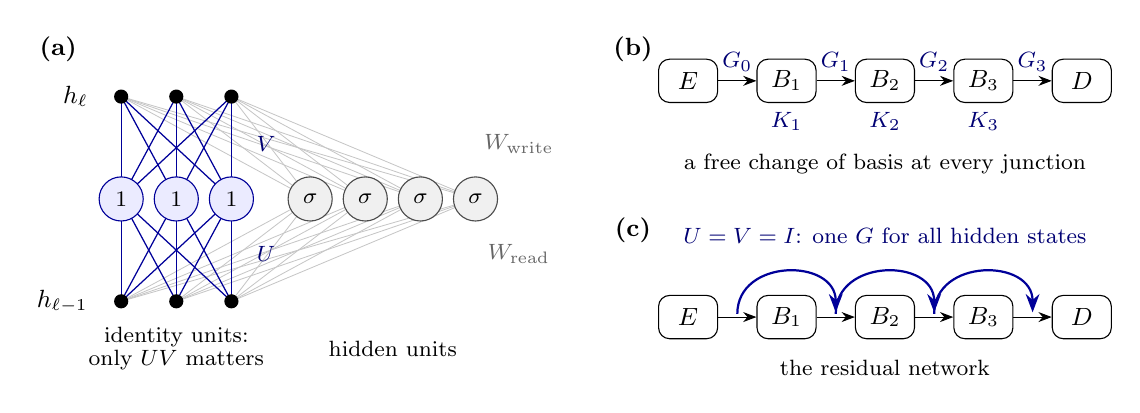
\begin{tikzpicture}[x=1mm,y=1mm,>=Stealth,
  blk/.style={draw,rounded corners,minimum width=7.5mm,minimum height=5.5mm,font=\small},
  lab/.style={font=\footnotesize,text=blue!45!black},
  panel/.style={font=\small\bfseries},
  io/.style={circle,fill=black,inner sep=0pt,minimum size=1.8mm},
  lin/.style={circle,draw=blue!60!black,fill=blue!8,minimum size=5.6mm,inner sep=0pt,font=\footnotesize},
  sig/.style={circle,draw=black!70,fill=gray!12,minimum size=5.6mm,inner sep=0pt,font=\footnotesize},
  idedge/.style={blue!60!black,line width=0.45pt},
  branchedge/.style={gray!45,line width=0.3pt}]
% (a) one mixed block as one wide layer
\node[panel] at (-4,40) {(a)};
\foreach \i/\x in {1/4,2/11,3/18} {
  \coordinate (in\i)  at (\x,8);
  \coordinate (lin\i) at (\x,21);
  \coordinate (out\i) at (\x,34);
}
\foreach \k/\x in {1/28,2/35,3/42,4/49} \coordinate (sg\k) at (\x,21);
\foreach \i in {1,2,3} \foreach \k in {1,...,4} {\draw[branchedge] (in\i)--(sg\k); \draw[branchedge] (sg\k)--(out\i);}
\foreach \i in {1,2,3} \foreach \j in {1,2,3} {\draw[idedge] (in\i)--(lin\j); \draw[idedge] (lin\j)--(out\i);}
\foreach \i in {1,2,3} {\node[io] at (in\i) {}; \node[io] at (out\i) {}; \node[lin] at (lin\i) {$1$};}
\foreach \k in {1,...,4} \node[sig] at (sg\k) {$\sigma$};
\node[anchor=east,font=\small] at (1,8)  {$h_{\ell-1}$};
\node[anchor=east,font=\small] at (1,34) {$h_{\ell}$};
\node[lab] at (22.4,14) {$U$};
\node[lab] at (22.4,28) {$V$};
\node[font=\footnotesize,text=black!60] at (54.5,14) {$\Wread$};
\node[font=\footnotesize,text=black!60] at (54.5,28) {$\Wwrite$};
\node[align=center,font=\footnotesize] at (11,2) {identity units:\\[-1pt] only $UV$ matters};
\node[align=center,font=\footnotesize] at (38.5,2) {hidden units};
% (b) a network of mixed blocks, without skips
\def\ox{76}
\node[panel] at ({\ox-7},40) {(b)};
\node[blk] (a0) at (\ox,36) {$E$};
\node[blk] (a1) at ({\ox+12.5},36) {$B_1$};
\node[blk] (a2) at ({\ox+25},36) {$B_2$};
\node[blk] (a3) at ({\ox+37.5},36) {$B_3$};
\node[blk] (a4) at ({\ox+50},36) {$D$};
\foreach \i/\j in {0/1,1/2,2/3,3/4} \draw[->] (a\i)--(a\j) node[midway,above,lab]{$G_{\i}$};
\foreach \i in {1,2,3} \node[lab] at ($(a\i)+(0,-5.2)$) {$K_{\i}$};
\node[font=\footnotesize] at ({\ox+25},25.5) {a free change of basis at every junction};
% (c) the gauge fixed: the residual network
\node[panel] at ({\ox-7},17) {(c)};
\node[blk] (b0) at (\ox,6) {$E$};
\node[blk] (b1) at ({\ox+12.5},6) {$B_1$};
\node[blk] (b2) at ({\ox+25},6) {$B_2$};
\node[blk] (b3) at ({\ox+37.5},6) {$B_3$};
\node[blk] (b4) at ({\ox+50},6) {$D$};
\foreach \i/\j in {0/1,1/2,2/3,3/4} \draw[->] (b\i)--(b\j);
\foreach \x in {12.5,25,37.5} \draw[->,thick,blue!60!black] ({\ox+\x-6.25},6.4) .. controls ({\ox+\x-6.25},13.5) and ({\ox+\x+6.25},13.5) .. ({\ox+\x+6.25},6.6);
\node[lab] at ({\ox+25},16.3) {$U = V = I$: one $G$ for all hidden states};
\node[font=\footnotesize] at ({\ox+25},-0.5) {the residual network};
\end{tikzpicture}
\caption{(a)~A mixed vanilla MLP block with $\dm = 3$ identity units and $4$ hidden units, drawn as one wide layer: its read places $U$ and $\Wread$ side by side, its map is $[\,\mathrm{Id}, \mathrm{Id}, \mathrm{Id}, \sigma, \sigma, \sigma, \sigma\,]$, and its write stacks $V$ and $\Wwrite$. Nothing nonlinear happens between the read $U$ and the write $V$ of the identity units, so only $UV$ enters the function (\cref{prop:junction}). (b)~A network of such blocks, or of blocks without identity units, between an embedding $E$ and a readout $D$: each hidden state has a free change of basis $G_\ell$, and the identity units of each block a free $K_\ell$. (c)~Spending them sets $U = V = I$ in every block, which is the residual network (\cref{thm:gauge}); the frozen identity units carry each hidden state into the next in the same basis, so one change of basis is left for all hidden states.}
\label{fig:junctions}
\end{figure}

\begin{table}[t]
\centering\footnotesize
\setlength{\tabcolsep}{3pt}
\caption{The main results, informally; \emph{Where} links to the precise statements. Networks have $L$ blocks (two per transformer layer) and hidden states of width $\dm$; $\G$ is the group of changes of basis at a hidden state. \emph{Support}: proof; measured, as the rank of a Jacobian on a batch of inputs (\cref{app:checks}); checked, by evaluating a construction in double precision; count, by arithmetic on released configurations; cited, proved by \citet{mijoski2026absorb}.}
\label{tab:results}
\newcolumntype{L}[1]{>{\raggedright\arraybackslash}p{#1}}
\begin{tabular}{@{}L{0.17\textwidth}L{0.16\textwidth}L{0.52\textwidth}L{0.1\textwidth}@{}}
\toprule
Result & Where & What it shows & Support \\
\midrule
Skips are gauge fixes & \cref{prop:junction}, \cref{thm:gauge} & Without normalization, trainable identity units and invertible learned skips reduce to identity skips, with the same functions and functional dimension; one global change of basis is left. & Proof, checked \\
\addlinespace[1pt]
Symmetry removed & \cref{cor:count}, \cref{sec:norm} & Against the skipless network with the same parameters, the skips remove $L\dim\G$ dimensions of symmetry: $L\dm^2$ without normalization; with $\varepsilon > 0$, $L\dm(\dm-1)/2$ under RMSNorm, $L(\dm-1)(\dm-2)/2$ under LayerNorm. & Proof \\
\addlinespace[1pt]
Identity units are new & \cref{thm:noabsorb} & Without biases, a block with identity units is not a block of the same kind and width without them: never for ReLU$^2$, ReGLU, SwiGLU and GeGLU, and for ReLU and GELU, with $\dm \ge 2$, only on a set of weights of measure zero. & Cited \\
\addlinespace[1pt]
Learned skips under RMSNorm & \cref{thm:rms} & Learned skips reduce to triangular or symmetric matrices; the identity skip fixes $\dm(\dm-1)/2$ dimensions of gauge and, under the equality condition, imposes $\dm(\dm+1)/2$ constraints. & Proof, checked, measured \\
\addlinespace[1pt]
Reduction without skips & \cref{prop:normalform} & One $\dm\times\dm$ block per hidden state becomes the identity, or triangular under normalization: $8.5$ percent of a skipless ViT-B. & Proof, count \\
\addlinespace[1pt]
One global change of basis & \cref{sec:global} & A symmetry outside the product of the groups of the blocks; with an untied readout it also removes one block, for example $0.03$ to $0.10$ percent of Llama-3.1. & Proof, checked, count \\
\addlinespace[1pt]
Gain, one block & \cref{thm:onelayer} & The skip adds exactly $\dm^2$ to the functional dimension ($\tanh$, GELU, ReLU, ReLU$^2$, ReGLU, attention), and under RMSNorm at least $\dm(\dm-1)/2$. & Proof, measured \\
\addlinespace[1pt]
Gain, deeper networks & \cref{fig:spectra}, \cref{sec:measured} & The gain equals the removed symmetry in $\tanh$, GELU and gated MLPs, with and without RMSNorm, and in nanoGPT, in every draw. & Measured \\
\addlinespace[1pt]
Skipless networks as limits & \cref{prop:limits} & Without biases or normalization, every skipless network is a limit of residual networks of the same widths, with an error of order $1/t$ when each write is scaled up by a power of $t$ and the next read down by as much. & Proof, checked \\
\bottomrule
\end{tabular}
\end{table}

% ===== sections/setup.tex =====
\section{Setup}\label{sec:setup}

\takeaway{A block is a read, a fixed map and a write. Every network here is a chain of blocks with $\dm$ identity units each: deleting them gives the network without skips, and freezing their weights at the identity gives the residual network.}

\para{Blocks.} The hidden state of a network is a matrix $h \in \R^{T\times \dm}$ with one row of width $\dm$ per token: the samples of a batch, or the tokens of a sequence in a transformer. A \emph{block} is a triplet $B = (\Wread, f, \Wwrite)$ of a trainable \emph{read} $\Wread \in \R^{\dm\times p}$, a fixed map $f : \R^{T\times p} \to \R^{T\times q}$ and a trainable \emph{write} $\Wwrite \in \R^{q\times \dm}$, and it maps $h$ to $B(h) = f(h\Wread)\Wwrite$. In a \emph{vanilla MLP} block, $p = q = m$ and $f = [\,\sigma, \dots, \sigma\,]$ applies an activation $\sigma$ to each of the $m$ hidden units, row by row. In a \emph{GLU} block \citep{shazeer2020glu}, $p = 2m$ and $q = m$: $f$ splits the coordinates of a row into gates $z_{\mathrm g}$ and values $z_{\mathrm v}$ and returns $g(z_{\mathrm g}) \odot z_{\mathrm v}$, with the gate function $g$ the sigmoid in GLU, $\max(z, 0)$ in ReGLU, GELU in GeGLU and $z/(1 + e^{-z})$ in SwiGLU. In an \emph{attention} block with $H$ heads of width $d_h$, the read holds the query, key and value projections, $f$ is the attention map, which mixes the rows, and the write is the output projection. A transformer layer consists of two blocks, so $L$ counts sub-blocks.

\para{Identity units.} Give a block $\dm$ more units whose activation is the identity, read with $U \in \R^{\dm\times \dm}$ and written with $V \in \R^{\dm\times \dm}$. The result is the \emph{mixed block}
\begin{equation}\label{eq:mixed}
\tilde B(h) \;=\; \underbrace{h\,U V}_{\text{identity units}} \;+\; \underbrace{f(h\Wread)\,\Wwrite}_{\text{the block } B} \;=\; \tilde f\big(h\,[\,U \mid \Wread\,]\big)\begin{bmatrix} V \\ \Wwrite \end{bmatrix},
\end{equation}
with $\tilde f\big(\big[\, u \;\big|\; z \,\big]\big) = \big[\, u \;\big|\; f(z) \,\big]$ for the input $u$ of the identity units and the input $z$ of $f$. For a vanilla MLP block, $\tilde f = [\,\mathrm{Id}, \dots, \mathrm{Id}, \sigma, \dots, \sigma\,]$ is the \emph{mixed activation}, with $\dm$ identities followed by $m$ copies of $\sigma$, and a residual block is a block of width $\dm + m$ in which $\dm$ units have the identity as activation and their read and write frozen at the identity matrix \citep[Section~4]{lin2018resnet}.

\para{Networks.} A network of $L$ mixed blocks has hidden states $h_0 = xE$ and $h_\ell = \tilde B_\ell(h_{\ell-1})$ for $\ell = 1, \dots, L$, and output $y = h_LD$, with an embedding $E \in \R^{d_{\mathrm{in}}\times \dm}$ and a readout $D \in \R^{\dm\times d_{\mathrm{out}}}$. Deleting the identity units gives the network \emph{without skips}, or \emph{skipless} network, $h_\ell = B_\ell(h_{\ell-1})$; freezing $U_\ell = V_\ell = I$ gives the \emph{residual} network, $h_\ell = h_{\ell-1} + B_\ell(h_{\ell-1})$; and merging $U_\ell$ and $V_\ell$ into $A_\ell = U_\ell V_\ell$ gives the network with \emph{learned skips}, $h_\ell = h_{\ell-1}A_\ell + B_\ell(h_{\ell-1})$. The skipless and the residual network have the same $P$ parameters, and the skipless network is our baseline. Biases may be added inside and after $f$, and then the embedding and the readout have biases too.

\para{Normalization.} In a \emph{pre-norm} network the read of every block, and the readout, see $N(h)$ instead of $h$, where $N$ is RMSNorm, which divides each row $h^{(t)}$ by $\sqrt{\norm{h^{(t)}}^2/\dm + \varepsilon}$; a learned gain after $N$ is folded into the next read. The identity units, which carry the skip, read $h$ itself. LayerNorm is RMSNorm after the projection that removes from each row its mean (\cref{prop:ln}), and we treat it that way.

\para{Changes of basis.} For an invertible $G$, the \emph{change of basis} $G$ at a hidden state $h_\ell$ replaces every matrix $W$ that writes $h_\ell$ ($V_\ell$ and $\Wwrite^{\ell}$, or $E$ if $\ell = 0$) by $WG$, and every matrix $W$ that reads it ($U_{\ell+1}$ and $\Wread^{\ell+1}$, or $D$ if $\ell = L$) by $G^{-1}W$. Through RMSNorm a read sees $N(hG)$, and $N(hG) = N(h)Q$ for all $h$ exactly when $G = cQ$ with $Q$ orthogonal and $c > 0$, where $c = 1$ if $\varepsilon > 0$ (\cref{lem:rms}); such a read is replaced by $Q^{-1}W$. We write $\G$ for the group of changes of basis that pass through the reads: $\GL(\dm)$ without normalization, $\Ort(\dm)$ under RMSNorm with $\varepsilon > 0$, and the scaled orthogonal matrices $\CO(\dm)$ when $\varepsilon = 0$. Biases add a translation at each hidden state, which the skips do not tie (\cref{lem:translations}). A block can also have \emph{symmetries inside}, which leave the hidden states alone: the rescalings of hidden units for positively homogeneous activations such as ReLU, of the values of a GLU unit, and in ReGLU of its gates as well, and in attention an invertible map per head between queries and keys and another between values and outputs. We write $s$ for their dimension, which is the same with and without skips.

\para{Functional dimension.} Let $F_\theta$ be the function computed at parameters $\theta \in \R^P$. Following \citet{grigsby2022functional}, the \emph{functional dimension} at $\theta$ is the largest rank of the Jacobian of $\theta \mapsto (F_\theta(x_1), \dots, F_\theta(x_n))$ over finite batches of inputs, and the \emph{redundancy} is $P$ minus it; \emph{generic} values are those taken on an open set of full measure. A symmetry changes $\theta$ without changing $F_\theta$, so the redundancy is at least the dimension of the symmetries, when no continuous family of them fixes the parameters (\cref{lem:free}). A network satisfies the \emph{equality condition} if at generic parameters the redundancy is exactly this dimension. It is a hypothesis: we prove it for networks with one block, without normalization and, for the residual network, under RMSNorm (\cref{thm:onelayer}), and measure it in deeper ones (\cref{sec:measured}).

% ===== sections/gauge.tex =====
\section{Skip connections are gauge fixes}\label{sec:gauge}

\takeaway{The identity units and the hidden states between blocks are linear junctions; spending their changes of basis turns trainable identity units into skip connections, and against the network without skips this removes the change of basis at every hidden state but one.}

\subsection{Junctions}\label{sec:junctions}

Nothing nonlinear happens between the read of the identity units and their write, nor, without skips, between the write into a hidden state and the reads of it: both are linear junctions, where only the products of the matrices on the two sides enter the function.

\begin{restatable}[Junctions]{proposition}{propJunction}\label{prop:junction}
\textup{(a)} In a mixed block, $(U, V) \mapsto (UK, K^{-1}V)$ preserves the function for every $K \in \GL(\dm)$.\\
\textup{(b)} In a skipless network, and in a network of mixed blocks, a change of basis in $\G$ at any hidden state preserves the function.\\
\textup{(c)} Changes of basis at different junctions commute. A skipless network therefore carries one copy of $\G$ per hidden state, and a network of mixed blocks one more copy of $\GL(\dm)$ per block.
\end{restatable}
\proofin{app:prf-junction}

Part (a) is the merge: a mixed block depends on $U$ and $V$ only through $A = UV$, so a network of mixed blocks is the network with learned skips $A_\ell$. Under RMSNorm the identity units still read the raw stream, so their junction keeps all of $\GL(\dm)$, and only the hidden states are restricted to $\G$. For vanilla MLP blocks without normalization, both parts are cases of Proposition~C.1 of \citet{zhao2023symmetries}, which turns every change of basis that passes through the activation of a hidden layer into a symmetry: part (a) with the mixed activation $\tilde f$ of \cref{eq:mixed}, which passes the matrices $\mathrm{diag}(K, I)$, since $\tilde f\big(\tilde z\,\mathrm{diag}(K, I)\big) = \tilde f(\tilde z)\,\mathrm{diag}(K, I)$, and part (b) with the identity as the activation at the hidden states. Under RMSNorm with $\varepsilon > 0$, part (b) for the skipless network is the case of the radial rescaling of their Example~C.6. For one hidden layer, no wider than the wider of its input and its output, their Theorem~3.3 also shows that the change of basis moves the parameters in $\dm^2$ independent directions for $\GL(\dm)$ and in $\dm(\dm-1)/2$ for $\Ort(\dm)$, and \cref{lem:free} extends this to deep networks.

\subsection{The gauge fix}\label{sec:gaugefix}

The changes of basis at the junctions bring the read and the write of every identity unit to the identity.

\begin{restatable}[Skip connections are gauge fixes]{theorem}{thmGauge}\label{thm:gauge}
In (a) and (b), consider networks without normalization. Write the parameters of a network of mixed blocks as $\theta = \big(E,\ (U_\ell, V_\ell, \Wread^{\ell}, \Wwrite^{\ell})_{\ell=1}^{L},\ D\big)$ and those of a residual network as $\theta' = \big(E',\ (\Wread'^{\ell}, \Wwrite'^{\ell})_{\ell=1}^{L},\ D'\big)$, and let $F_\theta$ and $F^{\mathrm{res}}_{\theta'}$ be the functions they compute. For $\theta$ with every $A_\ell = U_\ell V_\ell$ invertible, set $\Lambda_\ell = A_{\ell+1} A_{\ell+2} \cdots A_L$ for $\ell = 0, \dots, L$, with $\Lambda_L = I$, and define
\[
\Phi(\theta) = \big(E\Lambda_0,\ (\Lambda_{\ell-1}^{-1}\Wread^{\ell},\ \Wwrite^{\ell}\Lambda_\ell)_{\ell=1}^{L},\ D\big).
\]
With biases, $\Phi$ also sends the embedding bias $b_E$ to $b_E\Lambda_0$ and each write bias $b^{\ell}_{\mathrm{write}}$ to $b^{\ell}_{\mathrm{write}}\Lambda_\ell$, and keeps each read bias.\\
\textup{(a)} The changes of basis $\Lambda_\ell$ at $h_\ell$, for $\ell = 0, \dots, L$, and $K_\ell = U_\ell^{-1}\Lambda_{\ell-1}$ at the identity units of block $\ell$ set every $U_\ell$ and $V_\ell$ to $I$, and every other parameter to its entry in $\Phi(\theta)$. Hence $F_\theta = F^{\mathrm{res}}_{\Phi(\theta)}$.\\
\textup{(b)} Every parameter of the residual network is $\Phi(\theta)$ for some $\theta$, and $\Phi(\theta) = \Phi(\theta')$ exactly when changes of basis $K_1, \dots, K_L$ at the identity units and $G_0, \dots, G_{L-1}$ at $h_0, \dots, h_{L-1}$, with $G_L = I$, take $\theta$ to $\theta'$. The Fr\'echet derivative $\Der_\theta\Phi(\theta)$ is onto at every $\theta$. So the networks of mixed blocks with invertible $A_\ell$ and the residual networks compute the same set of functions, and at $\theta$ and $\Phi(\theta)$ they have the same functional dimension. For learned skips, with parameters $\big(E, (A_\ell, \Wread^{\ell}, \Wwrite^{\ell})_{\ell=1}^{L}, D\big)$, the same holds with the same formula for $\Phi$ and the changes of basis $G_\ell$ alone.\\
\textup{(c)} With or without RMSNorm, if every block is nonzero for some value of its parameters, changes of basis $G_0, \dots, G_L$ in $\G$ at the hidden states preserve the function of the residual network for all values of its parameters if and only if $G_0 = G_1 = \dots = G_L$.
\end{restatable}
\proofin{app:prf-gauge}

\para{The sweep.} The change of basis at the identity units sets $V_\ell = I$ but leaves the skip $A_\ell = U_\ell V_\ell$ unchanged. The skip changes only through the changes of basis at the two hidden states that it joins, $A_\ell \mapsto G_{\ell-1}^{-1}A_\ell G_\ell$, and each of these also acts on the neighbouring skip, so all of them must be chosen together. We therefore propagate a change of basis through the skips, from the readout back: a skip becomes the identity when $G_{\ell-1} = A_\ell G_\ell$, and $G_L = I$ gives $G_\ell = \Lambda_\ell$. Every chain of invertible skips thus has the form $A_\ell = \Lambda_{\ell-1}\Lambda_\ell^{-1}$ that the changes of basis $\Lambda_\ell^{-1}$ produce from identity skips. The product of all skip matrices ends up in the embedding, or, run from the embedding forward, in the readout (\cref{app:prf-gauge}). Part (b) says that the gauge fix loses nothing.

\para{Why one change of basis is left.} Part (c) is the tie. After changes of basis at $h_{\ell-1}$ and $h_\ell$ the branch becomes $B_\ell(\,\cdot\,G_{\ell-1}^{-1})\,G_\ell$, and the residual update computes
\begin{equation}\label{eq:defect}
h_{\ell-1}G_{\ell-1} + B_\ell(h_{\ell-1})\,G_\ell \;=\; h_\ell\,G_\ell \;+\; h_{\ell-1}\,(G_{\ell-1} - G_\ell).
\end{equation}
The frozen identity units carry $h_{\ell-1}$ in the basis $G_{\ell-1}$, and the branch writes in the basis $G_\ell$; unless the two agree, the defect $h_{\ell-1}(G_{\ell-1} - G_\ell)$ is passed on to every later block. In the language of gauge theory, the change of basis of a skipless network is local in depth, and the frozen identity units restrict it to a global one \citep{hashimoto2024unification}.

\para{When the block dominates the skip.} The defect is carried by the skip: relative to $h_\ell G_\ell$ it is at most $\norm{h_{\ell-1}}\norm{G_{\ell-1} - G_\ell}/\norm{h_\ell G_\ell}$, which is small where the branch dominates, $\norm{B_\ell(h_{\ell-1})} \gg \norm{h_{\ell-1}}$. There changes of basis that differ only across this block are approximate symmetries, and the residual block differs from its branch alone by a relative $\norm{h_{\ell-1}}/\norm{B_\ell(h_{\ell-1})}$, although in general no skipless block of the same kind and width equals it exactly (\cref{sec:oneblock}). The optimizer ARO shares one rotation through the skips, as the exact symmetry requires, and relaxes it to one rotation per transformer layer where the skips are weak \citep[Section~6.4]{gong2026aro}. In our check, a change of basis at every hidden state after one block, so that only the skip of that block joins two bases, changes the output by a relative $0.25$ when the branch is about half the size of the skip, and by $5\times10^{-3}$ when it is about fifty times larger (\cref{app:checks}).

\subsection{What the skips remove}\label{sec:count}

\begin{restatable}[What the skips remove]{corollary}{corCount}\label{cor:count}
The changes of basis form a group of dimension $(L+1)\dim\G$ in a skipless network and $\dim\G$ in a residual one, so the $L$ skips remove $L\dim\G$ dimensions of symmetry. Suppose that in both networks no continuous family of these symmetries and of those inside the blocks fixes generic parameters, which holds in MLP networks and transformers when the embedding has rank $\dm$ and every block has width at least $\dm$ (\cref{lem:free}, \cref{rem:attnfree}). Then:\\
\textup{(a)} the functional dimension is at most $P - (L+1)\dim\G - s$ without skips and at most $P - \dim\G - s$ with them;\\
\textup{(b)} under the equality condition for both networks, the skips raise the functional dimension by exactly $L\dim\G$, which is $L\dm^2$ without normalization.
\end{restatable}
\proofin{app:prf-count}


\para{Parameter counts understate residual networks.} \Cref{tab:ledger} in \cref{app:prf-count} keeps the books. The identity units of a block add $2\dm^2$ parameters and $\dm^2$ dimensions of symmetry, so on balance $\dm^2$ of functional dimension, and the gauge fix removes their $2\dm^2$ parameters together with $2\dm^2$ dimensions of symmetry. With biases every hidden state also carries a translation, and the gain is again $L\dm^2$ (\cref{lem:translations}). Under the equality condition the residual network thus has functional dimension $P - \dim\G - s$ and the skipless one $P - (L+1)\dim\G - s$. At equal parameter count the residual network has $L\dim\G$ more independent directions in function space, $L\dm^2$ without normalization and $L\dm(\dm-1)/2$ under RMSNorm; in this sense a residual network with $P$ parameters is worth a skipless one with $P + L\dim\G$, and the skipless network can shed its surplus after training (\cref{sec:skipless}). Comparisons at equal parameter count therefore favor residual networks. A fair comparison matches functional dimension instead and gives the skipless network $L\dim\G$ more parameters, $L\dm^2$ without normalization and about $L\dm^2/2$ with it: $7.1$M, or $8.1$ percent, for the skipless ViT-B of \citet{ji2026cutting} against the residual one (\cref{sec:skipless}).

\subsection{Are the identity units new?}\label{sec:oneblock}

The gain needs identity units that the other units of a block cannot absorb. A linear branch absorbs them: $h + hA = h(I + A)$, the deep linear residual network of \citet{hardt2017identity}, whose identity parametrization adds no functional dimension. So do $2\dm$ more ReLU, GELU or SiLU units, since $\sigma(z) - \sigma(-z) = z$. At the same width, \citet{mijoski2026absorb} show that the common blocks cannot; we restate their results in our notation. A block is \emph{nondegenerate} if the columns of $\Wread$ are nonzero and pairwise non-collinear and the rows of $\Wwrite$ are nonzero.

\begin{theorem}[{\citealp{mijoski2026absorb}}]\label{thm:noabsorb}
Let $B$ be a vanilla or GLU MLP block without biases (\cref{sec:setup}), of width $m \ge \dm$, let $M \neq 0$ be a $\dm \times \dm$ matrix, and ask for a block $B'$ of the same kind and width, that is, with the same activation or the same gate function and $m$ hidden units but any read and write, also without biases, such that $xM + B(x) = B'(x)$ for all row vectors $x \in \R^{1\times \dm}$.\\
\textup{(a)} If the blocks are positively homogeneous of degree $k > 0$, $k \neq 1$, as ReLU$^2$ and ReGLU blocks are, there is none (their Proposition~5).\\
\textup{(b)} If the blocks are gated with a gate that is differentiable at $0$ and vanishes there, as SwiGLU and GeGLU blocks are, there is none (their Proposition~6).\\
\textup{(c)} If $\sigma$ is ReLU or GELU, $\dm \ge 2$, $M = I$ and $B$ is nondegenerate, then $B'$ exists if and only if $\Wread[{:},S]\,\Wwrite[S,{:}] = -I$ for some set $S$ of hidden units, and for almost all weights it does not (their Theorems~8 and~10 and Corollary~11). For an invertible $M$ the same holds with $-M$ in place of $-I$ (their Lemma~4).\\
\textup{(d)} For blocks as in (a) with $k > 1$ or as in (b), no composition of $L$ residual blocks $x \mapsto x + B_\ell(x)$ equals a composition of $L$ blocks without skips of the same width (their Corollary~7).
\end{theorem}

Here $\Wread[{:},S]$ and $\Wwrite[S,{:}]$ keep the columns and the rows of the units in $S$. Parts (a), (b) and (d) compare how the two sides scale along rays from the origin. In part (c) the even part of the activation matches the hidden units of the two blocks up to sign and scale, and its odd part, $z/2$, turns a sign flip into a linear term, as \citet[Section~3]{petzka2020symmetries} show for two-layer ReLU networks with one output. So a residual block is not a block of the same kind and width without a skip: never in cases (a) and (b), and for almost all weights in case (c). In cases (a) and (b) the identity units of a mixed block are determined by its function: if two mixed blocks of the same kind and width compute the same function, the difference $M$ of their merged matrices satisfies $xM + B(x) = B'(x)$, so $M = 0$. The merge of \cref{prop:junction}(a) is then the only continuous symmetry that the identity units add, and the gauge fix of \cref{thm:gauge} is well defined.

% ===== sections/norm.tex =====
\section{Under normalization: triangular skips}\label{sec:norm}

\takeaway{Only orthogonal changes of basis pass through RMSNorm, so a skip matrix splits into an orthogonal part, which is gauge, and a triangular or symmetric part, which is not: the identity skip fixes the first and constrains the second.}

Under normalization the identity units, which carry the skip, read $h$, while the block reads $N(h)$. We therefore start from the network with learned skips
\begin{equation}\label{eq:prenorm}
h_\ell = h_{\ell-1}A_\ell + f_\ell\big(N(h_{\ell-1})\,\Wread^{\ell}\big)\,\Wwrite^{\ell},\qquad y = N(h_L)\,D.
\end{equation}
A change of basis at $h_\ell$ must now pass through $N$, so it lies in $\G$, which is $\Ort(\dm)$ for $\varepsilon > 0$ (\cref{lem:rms}), while the skip matrices, which read the raw stream, absorb any change of basis: $A_\ell \mapsto G_{\ell-1}^{-1}A_\ell G_\ell$.

\begin{restatable}[RMSNorm: a gauge fix and a constraint]{theorem}{thmRMS}\label{thm:rms}
Consider pre-RMSNorm networks with $\varepsilon > 0$, and the network with learned skips of \cref{eq:prenorm}.\\
\textup{(a)} If every $A_\ell$ is invertible, orthogonal changes of basis at $h_1, \dots, h_L$ turn every $A_\ell$ into an upper triangular matrix $R_\ell$ with positive diagonal, or alternatively into a symmetric positive definite matrix $S_\ell$. Recursively, with $Q_0 = I$, write $Q_{\ell-1}^\top A_\ell = R_\ell Q_\ell^\top$, an RQ factorization, or $Q_{\ell-1}^\top A_\ell = S_\ell Q_\ell^\top$, a polar decomposition, with $Q_\ell$ orthogonal, and apply $Q_\ell$ at $h_\ell$.\\
\textup{(b)} Let every $A_\ell$ be invertible and $\Pi_\ell = A_1\cdots A_\ell$, with $\Pi_0 = I$. If every $\Pi_\ell$ is orthogonal, the changes of basis $\Pi_\ell^{-1}$ at $h_\ell$ turn the network into the pre-RMSNorm residual network with embedding $E$, reads $\Pi_{\ell-1}\Wread^{\ell}$, writes $\Wwrite^{\ell}\Pi_\ell^{-1}$ and readout $\Pi_LD$, which computes the same function. If the reads and the readout have rank $\dm$, changes of basis turn the network into a pre-RMSNorm residual network with the same function only if every $\Pi_\ell$ is orthogonal.\\
\textup{(c)} Under the equality condition for the pre-RMSNorm networks with learned skips, with identity skips and without skips, the functional dimension of the network with learned skips exceeds that of the residual network by $L\,\dm(\dm+1)/2$, and that of the residual network exceeds that of the skipless network by $L\,\dm(\dm-1)/2$.\\
For $\varepsilon = 0$ the same holds with $\CO(\dm)$ in place of $\Ort(\dm)$, with the orthogonal factors of the $\Pi_\ell$ in the reads and the readout of (b), and the two differences in (c) become $L\,(\dm(\dm+1)/2 - 1)$ and $L\,(\dm(\dm-1)/2 + 1)$.
\end{restatable}
\proofin{app:prf-rms}

\para{The identity skip is a gauge fix and a constraint.} Of the $\dm^2$ entries of a skip matrix $A = RQ$, the $\dm(\dm-1)/2$ of the orthogonal factor $Q$ are gauge: changes of basis remove them exactly (part (a)). The $\dm(\dm+1)/2$ of the triangular factor $R$, or of the symmetric factor $S$ in $A = SQ$, are not, and under the equality condition setting them to the identity lowers the functional dimension by as much (part (c)), which we measure at $\dm = 4$ and $L = 3$ (\cref{app:checks}). So under RMSNorm an identity skip fixes the gauge at a hidden state and also imposes $\dm(\dm+1)/2$ constraints; without normalization it only fixes the gauge. Rotations in the skips are pure gauge: SliceGPT inserts them before it deletes rows and columns \citep[Sections~3.3 and~3.4]{ashkboos2024slicegpt}, and \citet[Section~4.6]{vannierop2024gauge} inserts them into LayerNorm transformers to recover one copy of the stream symmetry per skip, at the cost of as many parameters.

\para{LayerNorm and DyT.} LayerNorm is RMSNorm after a projection: $\mathrm{LN}(h) = \gamma \odot N(hZ) + \beta$, with $Z$ the projection that removes the mean, so a LayerNorm network does not use the direction of the all-ones vector and normalizes the other $\dm - 1$ \citep{ashkboos2024slicegpt,theus2025glmc,baroni2026lnfree}. Folding the gains into the next reads and centring every write turns it into an RMSNorm network of width $\dm - 1$ (\cref{prop:ln}), with $\Ort(\dm-1)$ at each hidden state, so the skips remove $L(\dm-1)(\dm-2)/2$ dimensions, as we measure in nanoGPT (\cref{sec:measured}). An elementwise read such as DyT, $\gamma \odot \tanh(\alpha h) + \beta$ with a learnable scalar $\alpha$ \citep{zhu2025dyt}, lets through only signed permutations and one positive scale, which $\alpha$ absorbs, so the skips remove only $L$ dimensions (\cref{app:checks}).


\para{Low-rank skips.} The low-rank version of LAuReL trains its skip matrix as $A = I + UV^\top$ with $U, V \in \R^{\dm\times r}$ \citep{menghani2024laurel}. Without normalization such a skip, when invertible, is a learned skip, and \cref{thm:gauge} removes all $2\dm r$ of its parameters. Under RMSNorm, making it triangular would give up the low rank, since a triangular matrix has $\dm(\dm+1)/2$ entries against the $2\dm r$ of the factors. The product itself offers a change of basis of width $r$: $(U, V) \mapsto (UK, VK^{-\top})$ leaves $UV^\top$ unchanged for every $K \in \GL(r)$, so $r$ rows of $U$ can be set to the identity, which removes $r^2$ parameters per skip. The redundancy we measure under RMSNorm is larger, $r(2r-1)$ per skip when $2r \le \dm$: rotations of the two hidden states that keep the skip within rank $r$ of the identity add $r(r-1)$ (\cref{app:checks}). Whether triangular or symmetric skips train better than full or low-rank ones is an empirical question left for future work; a trained full skip can always be reduced afterwards (\cref{sec:learned}).

% ===== sections/reduce.tex =====
\section{Exact reduction after training}\label{sec:reduce}

\takeaway{Every change of basis that a trained network keeps can be spent on structure without changing its function: one block per hidden state without skips, one block in all with them, and the orthogonal part of every learned skip.}

\subsection{Without skips: one block per hidden state}\label{sec:skipless}

At a hidden state $h_\ell$, pick an invertible $\dm \times \dm$ block $W_1$, formed by $\dm$ columns of a matrix that reads $h_\ell$ or by $\dm$ rows of a matrix that writes it.

\begin{restatable}[One free block per hidden state]{proposition}{propNormalForm}\label{prop:normalform}
In a skipless network or a network of mixed blocks, let $W_1$ be an invertible $\dm \times \dm$ block formed by $\dm$ columns of a matrix that reads a hidden state $h_\ell$, or by $\dm$ rows of a matrix that writes it. Without normalization, a change of basis at $h_\ell$ turns $W_1$ into the identity: $G = W_1$ for a read and $G = W_1^{-1}$ for a write. Under RMSNorm with $\varepsilon > 0$, an orthogonal change of basis at $h_\ell$ turns $W_1$ into a triangular matrix: for a read, write $W_1 = QT$ with $Q$ orthogonal and $T$ upper triangular, the QR factorization of $W_1$, and take $G = Q$; for a write, write $W_1 = TQ$ with $T$ lower triangular, from the QR factorization of $W_1^\top$, and take $G = Q^\top$. This can be done at every hidden state at once, and removes $\dm^2$, respectively $\dm(\dm-1)/2$, parameters per hidden state without changing the function. In a residual network the hidden states share one change of basis, which does the same for a single such block in the whole network, in any one read or write.
\end{restatable}
\proofin{app:prf-normalform}

On a skipless pre-RMSNorm network with $\dm = 16$ and $L = 4$ the reduction zeroes $8.1$ percent of the parameters and changes the function by a relative $1.8\times10^{-15}$; on a residual network the same step changes it by $1.5$, because there the hidden states share one change of basis.

\para{Three patterns.} A transformer layer without skips has two hidden states, before its attention block and before its MLP block, and each can fix one block. (i) \emph{Queries and output projections}, when $Hd_h = \dm$: $G = W_Q$ sets the queries to the identity and moves $W_Q$ into the write of the block before, and $G = W_O^{-1}$ sets the output projection to the identity and moves $W_O$ into the read of the next MLP block. This is how \citet{graef2024tricks} removes $2\dm^2$ parameters per layer in transformers without skips or normalization, fifteen percent of the weights of a skipless version of Mistral-7B by his count. Any $\dm$ columns of a read that form an invertible matrix will do instead, for instance some queries, some keys and some values. (ii) \emph{MLP blocks only}: $\dm$ columns of the read of each MLP block and $\dm$ rows of its write are set to the identity, absorbed by the attention blocks around it, which stay full; again $2\dm^2$ parameters per layer. (iii) \emph{Under normalization} the change of basis must be orthogonal, and the chosen block becomes triangular instead: $\dm(\dm-1)/2$ parameters per hidden state.

\para{A skipless Vision Transformer.} \citet{ji2026cutting} train a ViT-B without skips that reaches $80.8$ percent on ImageNet-1k with the optimizer SOAP \citep{vyas2025soap}, against $80.1$ percent for the residual ViT-B. Assuming standard pre-LayerNorm blocks, which \cref{prop:ln} turns into RMSNorm of width $\dm - 1 = 767$, each of its $25$ hidden states carries a free $\Ort(767)$, and one triangular $767 \times 767$ read block at each zeroes $25 \cdot 767 \cdot 766/2 = 7.3$M parameters, $8.5$ percent of the model, without changing its function. Against the residual ViT-B, which has the same parameters, it carries $24$ more copies of $\Ort(767)$, $7.1$M dimensions of symmetry (\cref{app:scale}), the parameters that a comparison at equal functional dimension would add to the skipless ViT-B (\cref{sec:count}). The saving is in memory if the triangular blocks are stored packed, and in compute only if triangular multiplies run at dense speed, for example in the rectangular full packed format of \citet{gustavson2010rfp}; measuring this is left for future work.

\subsection{With skips: one global change of basis}\label{sec:global}

A residual network keeps one change of basis for all its hidden states (\cref{thm:gauge}(c)). With the embedding and the readout as parameters, it is a symmetry of the whole model, with two consequences.

\para{A counterexample.} \citet{wang2025gauge} characterize the symmetries of transformer blocks and state that the symmetry group of a full transformer is the product of the groups of its blocks, since residual connections and LayerNorm prevent any coupling across layers (their Theorem~7). When the embedding and the readout are among the parameters, as in the models they name and in their end-to-end checks, the change of basis that the skips leave gives counterexamples. Applied at every hidden state from the embedding to the readout, a global permutation of the stream coordinates preserves the function for every placement of the normalization and with a tied or an untied readout, as \citet[Section~3.3]{verma2024merging} use to merge BERT models, and in pre-norm models with an untied readout so does a global rotation, the construction behind Theorem~1 of \citet{ashkboos2024slicegpt}. Both change the token embedding, which no element of the product of per-block groups does, so both lie outside that product (\cref{app:product}, \cref{tab:product}). For a bare stack of blocks that acts on a fixed input and is read in fixed coordinates, both change the function, and the counterexample does not apply.

\para{What it also removes.} The same change of basis can fix one block in the whole model, in any one read or write and at any depth (\cref{prop:normalform}). In a pre-RMSNorm model with an untied readout it makes one $\dm \times \dm$ block triangular and removes $\dm(\dm-1)/2$ parameters. We take Llama-3.1 as an example, a family with grouped-query attention \citep{grattafiori2024llama3}: the reduction removes $8.4$M parameters in Llama-3.1-8B, $34$M in Llama-3.1-70B and $134$M in Llama-3.1-405B, that is $0.10$, $0.05$ and $0.03$ percent (\cref{tab:scale}). The same holds for other pre-RMSNorm language models with multi-head or grouped-query attention and an untied readout, while multi-head latent attention, which computes keys and values from a shared low-rank latent through trainable up-projections \citep[Section~2.1.1]{deepseek2024v3}, is beyond the scope of this paper. The reduction is exact, but small; the interest of this symmetry is the counterexample above.

\para{Tied readouts.} With a tied readout, the readout $E^\top$ reads $h_L$ through the gain $g$ of the final normalization, and a global rotation $Q$ must keep one matrix $E$ at both ends, which requires $Q\,\mathrm{diag}(g')\,Q^\top = \mathrm{diag}(g)$ for some gain $g'$; for distinct gains only signed permutations do so. One $\dm \times \dm$ matrix inserted between the final normalization and the readout restores the rotations and absorbs the gain, but it costs $\dm^2$ parameters and frees only $\dm(\dm+1)/2$: for identity skips it does not pay (\cref{app:checks}).

\subsection{Learned skips after training}\label{sec:learned}

Networks trained with learned skips reduce exactly after training. Without normalization every invertible skip matrix is removed, the product of all of them moves into the embedding or the readout (\cref{thm:gauge}), and the change of basis that is left fixes one more block, in any one read or write (\cref{prop:normalform}). Under RMSNorm every skip becomes triangular or symmetric positive definite (\cref{thm:rms}(a)), which removes $\dm(\dm-1)/2$ parameters per skip; started at any hidden state instead of $h_0$, the recursion also makes one block of a read or a write of that state triangular (\cref{app:prf-rms}). With a tied readout under RMSNorm, the embedding also reads $h_L$, which fixes the rotations at $h_0$ and $h_L$, for generic gains up to signs and permutations; those at $h_1, \dots, h_{L-1}$ stay free. They make any $L - 1$ of the skips triangular, and the remaining one keeps its full matrix: $(L-1)\dm(\dm-1)/2$ parameters are removed. One more $\dm \times \dm$ matrix inserted before the readout frees the rotations at $h_0$ and $h_L$ and absorbs the gain, $\dm(\dm-1)/2 + \dm(\dm-1)/2 + \dm = \dm^2$ parameters, exactly its cost: it does not pay. Without normalization the tie only requires $G_L = G_0^{-\top}$: any $L - 1$ of the skips become identities, and the free $G_0$ sets one block of any one read or write to the identity, which removes $L\dm^2$ parameters. At $\dm = 8$ and $L = 5$ the function changes by $5\times10^{-16}$ for triangular skips, $4\times10^{-15}$ for symmetric ones and $7\times10^{-16}$ with a tied readout, where $112$ parameters are removed (\cref{app:checks}). Low-rank skips are removed entirely without normalization, and give up at least the $r^2$ parameters inside the product under RMSNorm (\cref{sec:norm}).

% ===== sections/gain.tex =====
\section{When the count is functional dimension}\label{sec:gain}

\takeaway{The symmetry removed by the skips is a gain in functional dimension when the symmetries are the only redundancy of both networks; we prove this for one block, attention included, and measure it in deeper MLPs and small transformers. In exchange the skips lose no function in the limit: every skipless network without biases or normalization is a limit of residual networks of the same widths.}

The gain of \cref{cor:count}(b) needs the equality condition, for the residual and for the skipless network. A \emph{ReLU$^2$} block \citep{so2021primer} uses $\sigma(z) = \max(z, 0)^2$, and a \emph{ReGLU} block \citep{shazeer2020glu} is the GLU block with the gate $\max(z, 0)$. The symmetries inside a block rescale its $m$ hidden units for ReLU and ReLU$^2$, so each block contributes $m$ to $s$, and gates and values separately for ReGLU, so each block contributes $2m$; $\tanh$ and GELU blocks contribute nothing. An attention block of $H$ heads of width $d_h$ contributes $2Hd_h^2$: in each head, a change of basis between queries and keys and one between values and outputs.

\begin{figure}[t]
\centering
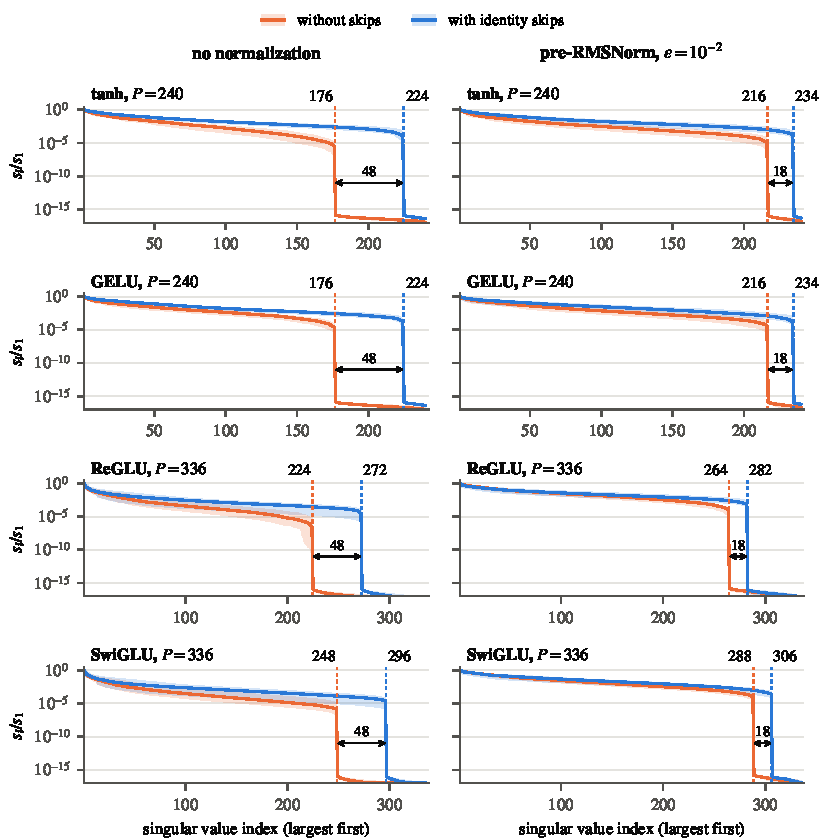
\includegraphics[width=\linewidth]{figs/spectra.pdf}
\caption{Singular values of the exact Jacobian of the parameter-to-output map, on $4000$ inputs, for the same weights with and without identity skips: an embedding $\R^6 \to \R^4$, $L = 3$ MLP blocks of width $8$ and a readout $\R^4 \to \R^6$, without biases. Left column: without normalization. Right column: with pre-RMSNorm, $\varepsilon = 10^{-2}$, before every block and the readout. Lines show the median over $20$ random draws, and bands the range. The rank on the batch is a lower bound on the functional dimension, and the symmetry count $P - (L+1)\dim\G - s$ without skips and $P - \dim\G - s$ with them an upper bound, with $\dim\G = \dm^2 = 16$ without normalization and $\dm(\dm-1)/2 = 6$ under RMSNorm; the dashed lines mark the two counts, and the arrows their difference. In every draw the rank, read at a gap of at least $10^4$, equals the count, so the skips add $L\dim\G$: $48$ without normalization and $18$ under RMSNorm.}
\label{fig:spectra}
\end{figure}

\subsection{One block}\label{sec:onelayer}

For networks with one block the equality condition is a theorem, except for the skipless network under RMSNorm, for which we prove only the bound of \cref{cor:count}(a) (\cref{thm:onelayer} in \cref{app:onelayer}). Let $\dm \ge 2$, and let the block have width at least $\dm$, with inputs and outputs of dimension at least $\dm$: a $\tanh$, GELU, ReLU, ReLU$^2$ or ReGLU block, or an attention block with heads of width at most $\dm$, causal or not, on sequences of at least two tokens. Without normalization, with or without biases, at generic parameters, the skipless and the residual network both satisfy the equality condition, so the skip raises the functional dimension by exactly $\dm^2$; for attention without biases this extends to a learned absolute position embedding. Under pre-RMSNorm with $\varepsilon > 0$, without biases, the residual network satisfies it too, and the skip adds at least $\dm(\dm-1)/2$.

The proof uses only linear algebra and limits in one variable. The parameters enter through $M = ED$, $A = \Wwrite D$ and $C = E\Wread$, as $x \mapsto f(xC)A$ without the skip and $x \mapsto xM + f(xC)A$ with it. A factorization of a rank-$\dm$ matrix into two factors of rank $\dm$ is unique up to an invertible $\dm \times \dm$ matrix between them, so the skipless network carries two changes of basis, and $M = ED$ ties them into one. It remains to show that a direction that leaves the function unchanged to first order moves $M$, $A$ and $C$ only along the symmetries of the hidden units, which are isolated by their kinks for the ReLU-type activations, with an argument of the kind \citet{mijoski2026absorb} use for ReLU blocks, and along rays by how fast they approach their limits for $\tanh$ and GELU. On inputs with two distinct tokens, the output of an attention block at the second token is a $\tanh$ network with one unit per head, since a softmax over two distinct scores is a logistic function of their difference.

\subsection{Deeper networks}\label{sec:measured}

For deeper networks we compute the rank of the Jacobian of the parameter-to-output map on a large batch of inputs (\cref{app:checks}). This rank is a lower bound on the functional dimension, and the symmetry count is an upper bound (\cref{cor:count}(a)). Where the two meet, the functional dimension is exactly the count, which is the equality condition.


\para{MLPs.} In the networks of \cref{fig:spectra} the two bounds meet in every draw, with and without RMSNorm: the singular values drop to the floor of double precision exactly at the count, so the skips add $L\dm^2$ without normalization and $L\dm(\dm-1)/2$ under RMSNorm. The measured redundancy also equals the symmetry count for $\tanh$ networks up to $\dm = 16$ and $L = 6$, with and without RMSNorm, and with biases at $\dm = 4$ (\cref{tab:checks}).

\para{Transformers.} We take the model of nanoGPT \citep{karpathy2023nanogpt} with $\dm = 8$, four heads of size two, a vocabulary and a context of $8$, and no biases, as its training script sets them, with a readout not tied to the embedding. We keep its LayerNorm or replace it by the identity, and removing both skips of each layer gives the skipless network with the same parameters. With $1$ to $4$ layers and $4$ random draws each, all $64$ networks have the predicted redundancy, and the skips add $L(\dm-1)(\dm-2)/2 = 21L$ with LayerNorm and $L\dm^2 = 64L$ without (\cref{tab:nanogpt}). The rest of the redundancy, the same with and without skips, comes from symmetries inside the heads and from LayerNorm; for one and two layers we construct all of them and find that they span the null space of the Jacobian.

\subsection{Skipless networks as limits of residual networks}\label{sec:limits}

Every skipless network is a limit of residual networks with the same widths, so the gain in functional dimension does not come at the price of functions. In this subsection the networks have no biases and no normalization.

\begin{restatable}[Skipless networks as limits of residual networks]{proposition}{propLimits}\label{prop:limits}
Let $S$ be a network without skips, biases or normalization, with embedding $E$, blocks $B_\ell(h) = f_\ell(h\Wread^{\ell})\Wwrite^{\ell}$ for $\ell = 1, \dots, L$ whose maps $f_\ell$ are locally Lipschitz, and readout $D$. For $t \ge 1$, let $F_t$ be the residual network with the embedding $E$, the reads $t^{1-\ell}\Wread^{\ell}$, the writes $t^{\ell}\Wwrite^{\ell}$ and the readout $t^{-L}D$. For every bounded set $X$ of inputs there is $C$ such that $\norm{F_t(x) - S(x)} \le C/t$ for all $x \in X$ and $t \ge 1$.
\end{restatable}
\proofin{app:prf-limits}

\para{Blocks that outweigh their skips.} Scaling the reads of block $\ell$ by $t^{1-\ell}$ and its writes by $t^\ell$ turns it into $h \mapsto t^\ell B_\ell(t^{1-\ell}h)$. Let $s_0 = xE$ and $s_\ell = B_\ell(s_{\ell-1})$ be the hidden states of $S$. If the hidden state of $F_t$ before block $\ell$ is $t^{\ell-1}(s_{\ell-1} + r_{\ell-1})$, the block sees $s_{\ell-1} + r_{\ell-1}$ and returns $t^\ell B_\ell(s_{\ell-1} + r_{\ell-1})$, which outweighs the skip by a factor $t$. The hidden states of $F_t$ are thus $t^\ell(s_\ell + r_\ell)$, with $r_0 = 0$ and
\begin{equation}\label{eq:limit-rec}
r_\ell \;=\; B_\ell(s_{\ell-1} + r_{\ell-1}) - B_\ell(s_{\ell-1}) \;+\; t^{-1}\,(s_{\ell-1} + r_{\ell-1}).
\end{equation}
The difference is at most a local Lipschitz constant of $B_\ell$ times $\norm{r_{\ell-1}}$, and the last term is $O(1/t)$, so $r_L = O(1/t)$ and $F_t(x) = t^{-L}\,t^{L}(s_L + r_L)D = S(x) + O(1/t)$.

\para{No activation sees a large argument.} The large constants sit in the writes, and each read divides by the size $t^{\ell-1}$ that the stream has reached, so block $\ell$ of $F_t$ evaluates $f_\ell$ at $(s_{\ell-1} + r_{\ell-1})\Wread^{\ell}$, the pre-activations of $S$ up to $O(1/t)$. A GELU, for instance, is evaluated where the GELU of $S$ is, not at large arguments, where it would act like a ReLU. Only the stream grows, to order $t^L$ before the readout, which divides by $t^L$. The construction keeps the widths and uses nothing about the blocks but local Lipschitz continuity, so it applies alike to $\tanh$, GELU, ReLU, ReLU$^2$, gated and attention blocks. Its weights diverge as $t \to \infty$: the proposition says which functions residual networks reach in the limit, not how to parametrize them for training. In our checks, at $\dm = 4$ and $L = 3$, the error of $F_t$ relative to the largest output of $S$ is below $10^{-2}$ at $t = 1000$ for $\tanh$, GELU, ReLU, SiLU, ReLU$^2$, GLU, ReGLU, SwiGLU, GeGLU and attention blocks, with $t$ times the error nearly constant (\cref{app:checks}).

\para{Weight decay.} In training, weight decay is usually applied to the matrices but not to the gains of RMSNorm; nanoGPT, for instance, decays only its matrices \citep{karpathy2023nanogpt}. It penalizes the diverging writes of $F_t$, and in a pre-RMSNorm network without biases the gains are then the only parameters that can grow without penalty. A gain $c$ multiplies the input of a read, so it puts a large constant before the activation, not after it. For positively homogeneous blocks, such as ReLU, ReLU$^2$ and ReGLU blocks, this only scales the output of the block, which can then outweigh its skip as in $F_t$. So can gated blocks with any gate, SwiGLU and GeGLU included: if the read splits into gates and values, $\Wread = [\,W_{\mathrm g} \mid W_{\mathrm v}\,]$, the read $[\,W_{\mathrm g}/c \mid W_{\mathrm v}\,]$ gives the gate its old argument on the input $cx$ and passes $c$ to the values, so the block returns $c\,B(x)$, with a gate read that is smaller, not larger. A vanilla GELU block has no such linear path. Its activation sees large arguments, where $\mathrm{GELU}(cz)/c \to \max(z, 0)$ as $c \to \infty$, so it can outweigh its skip through its gains only by acting as a ReLU block, or with a large write, which weight decay penalizes. This is where GELU breaks, and so does SiLU.

% ===== sections/related.tex =====
\section{Related work}\label{sec:related}

\para{Changes of basis at hidden layers.} \citet{zhao2023symmetries} define a change of basis at every hidden layer of an MLP, which preserves the function where the activation there is linear and, for orthogonal changes, where it is a radial rescaling (their Proposition~C.1 with Examples~C.3 and~C.6). For one hidden layer they compute the dimension of the set of parameters that it reaches (their Theorem~3.3) and the conserved quantities of gradient flow, and use both to study extended flat minima. They remark that Proposition~C.1 adapts to networks with skip connections (their Appendix~C.5); what the skips do to the symmetry is not worked out there. Written as $\dm$ trainable units with the identity as activation, next to the hidden units of a vanilla MLP block without normalization, a skip fits their proposition as it stands, and propagating a change of basis through the skips, the tool of our gauge fix, is their change of basis at the identity units combined with those at the two hidden states that each skip joins (\cref{app:prf-gauge}). We use the same tool for a different result: the tie of \cref{thm:gauge}(c), the count of \cref{cor:count}, and the reductions of \cref{sec:reduce}. \citet{godfrey2022symmetries} characterize the linear maps that pass through an elementwise activation, and show that in residual ReLU networks permutations and positive rescalings of hidden units preserve the function when they are equal at all hidden states that the residual connections join (their Remark~3.6 and Appendix~E.9.2).

\para{The basis of the residual stream.} \citet{elhage2021circuits} observe that the residual stream has no privileged basis. \citet{ashkboos2024slicegpt} prove that an RMSNorm transformer computes the same function after one orthogonal transformation of every weight matrix touching the stream, a rotation that the skips propagate from the embedding to the readout (their Section~3.1 and Theorem~1). QuaRot and SpinQuant use the same invariance for quantization \citep{ashkboos2024quarot,liu2024spinquant}, model merging aligns residual streams with one global orthogonal matrix \citep{theus2025glmc}, and \citet{sweeney2026transport} studies the residual coordinates when normalization gains are kept as parameters; all of these use the one global change of basis that a residual network keeps. To sparsify trained models, SliceGPT rotates each block by the principal components of the signals between blocks on calibration data, inserts $Q_{\ell-1}^\top Q_\ell$ into each skip so that neighbouring blocks can carry different rotations, and deletes the rows and columns that correspond to the minor principal components (their Sections~3.3 and~3.4). The sparsity is structured: every weight matrix becomes a smaller dense matrix, and the sliced model approximates the original one. We propagate changes of basis through the skips in the opposite direction: SliceGPT inserts matrices into identity skips, while we remove the matrices of learned skips without changing the function. \citet[Sections~4.4 and~4.5]{vannierop2024gauge} counts the symmetries of LayerNorm transformers, with one rotation of the stream for the whole model; what the skips remove is of order $L\dm^2$ against his $L\dm d_h + \dm^2$, $7.1$M against $1.5$M in ViT-B/16 (\cref{app:scale}).

\para{Removing weights without skips.} \citet{graef2024tricks} merges the query and the output projection of every layer of a skipless transformer into its neighbours, the first of our three patterns. \citet{he2024simplifying} fix the value and projection matrices of skipless attention blocks to the identity without performance degradation, while with the attention skip identity values and projections hurt (their Figure~23), and they write that they do not have a satisfying explanation. In our terms, a change of basis reaches identity values in a skipless network (\cref{prop:normalform}), while with the skip the hidden states share one change of basis and identity values constrain the function. RMNet removes the skips of trained convolutional networks by emulating the identity with ReLU or PReLU units \citep{meng2021rmnet}, at the cost of more units, and LAuReL trains learned skips of low rank \citep{menghani2024laurel}.

\para{Symmetries and residual networks in theory.} \citet{wang2025gauge} characterize the symmetries of attention and MLP blocks; their statement for the full model has the counterexamples of \cref{sec:global}. \citet{marcotte2025resnets} show that a block has the same conservation laws of gradient flow with and without its skip (their Proposition~3.2). Likewise, without embedding or readout the skip does not change the derivative of a block with respect to its parameters, so the gain needs junctions outside the block, such as an embedding and a readout. \citet{mijoski2026absorb} ask when a one-hidden-layer block with an identity skip equals a block of the same width without one, and we restate their answer in \cref{thm:noabsorb}. \citet{lin2018resnet} count the identity map as $\dm$ hidden units, the view we take throughout, and \citet{macdonald2023skip} show that identity skips around contractive branches keep the Jacobian of the parameter-to-output map of full row rank on linearly independent inputs, which gives global convergence of gradient descent for residual networks with normalized weights; we study the kernel of the same Jacobian.

% ===== sections/outlook.tex =====
\section{Scope and future work}\label{sec:outlook}

\para{What is proved, measured and conjectured.} The gauge fixes of \cref{thm:gauge,thm:rms,prop:normalform}, the count of \cref{cor:count}, the reductions of \cref{sec:reduce} and the limits of \cref{prop:limits} hold for every network of the stated kind. That the count is a gain in functional dimension is proved for networks with one block, attention included, and measured in deeper MLPs and small transformers. For deeper networks it rests on the equality condition, which can fail: for ReLU networks the functional dimension varies on sets of positive measure \citep{grigsby2023hidden}, and some skipless networks are more redundant than their symmetries (\cref{app:checks}). We expect it for the common blocks:

\begin{conjecture}[Equality condition]\label{conj:equality}
Consider networks without biases whose embedding is linear in continuous inputs, with input and output dimensions at least $\dm$ and blocks of width at least $\dm$ that are all vanilla MLP blocks with $\tanh$ or GELU activations, or all SwiGLU, all GeGLU or all ReGLU blocks, without normalization or with pre-RMSNorm and $\varepsilon > 0$. At generic parameters the skipless and the residual network both satisfy the equality condition, so the skips raise the functional dimension by exactly $L\dim\G$.
\end{conjecture}

\para{Beyond the scope of this paper.} Input-dependent skips, such as the hyper-connections of mHC \citep{xie2025mhc} and DeepSeek-V4 \citep{deepseek2026v4}, which mix several streams with weights computed in part from the stream itself, make the junction between blocks nonlinear and are beyond the scope of this paper. So are quantized weights, whose grid a change of basis does not preserve, and streams that pass through an elementwise nonlinearity, as in the original ResNet \citep{he2016resnet}, which keep only permutations and positive rescalings at each hidden state.

\para{Training in the reduced forms.} Our claim is about trained networks: in the worst case, the reductions of \cref{sec:reduce} are applied after training, where they lower the memory of the model exactly. Whether they also help during training is left for future work. Two direct tests are to train a skipless network in the reduced parametrization of \cref{prop:normalform} against the full one, and to train learned skips under RMSNorm in their triangular or symmetric form (\cref{thm:rms}) against full and low-rank ones. Optimizers already use the rotations of the stream: ARO can share one rotation among all matrices that read or write the stream, as the global symmetry allows, or one per transformer layer, a relaxation that it motivates where the output of a layer outweighs its skip \citep[Sections~6.4 and~6.5]{gong2026aro}.

\para{Orthogonal or symmetric skips, at depth and at width.} Under RMSNorm the two parts of a learned skip do different things (\cref{sec:norm}). Orthogonal skips are gauge: a network with orthogonal skips computes the function of a residual network whose hidden states have the same norms (\cref{thm:rms}(b)), so they can change how the network trains but not what it computes. With them, a separate rotation at every hidden state is an exact symmetry; with identity skips it holds only approximately, where the branch outweighs the skip (\cref{sec:gaugefix}), the regime in which ARO uses one rotation per layer \citep[Section~6.4]{gong2026aro}. They also let each block see the stream in a basis of its own, which matters to optimizers that act on each coordinate separately. Symmetric or triangular skips carry what learned skips add to the functional dimension, $\dm(\dm+1)/2$ per skip under the equality condition (\cref{thm:rms}(c)), and they change norms: the output of block $\ell$ reaches $h_L$ multiplied by $A_{\ell+1}\cdots A_L$, which keeps its norm when the skips are orthogonal and can otherwise damp or amplify it geometrically with depth. At width, both kinds cost about $\dm^2/2$ parameters per skip, and a full skip spends $\dm(\dm-1)/2$ of its $\dm^2$ parameters, a share that approaches one half, on its orthogonal part. Whether orthogonal or symmetric and triangular skips bring more value, per parameter and per unit of compute, as depth and width grow, is left for future work.

\para{Continuous depth.} \citet{geshkovski2025transformers} model a transformer as a flow in continuous time: the layers become time, the tokens interacting particles, and layer normalization, with its gain set to the identity, keeps them on the sphere. Their view follows the neural ODEs of residual networks, in which the skip is what makes a layer an Euler step, and what the gauge fix becomes in this limit is an open question. In a flow, a change of basis $h \mapsto hG(t)$ at every time adds the linear term $h\,G^{-1}G'$ to the velocity field, where $G' = \mathrm{d}G/\mathrm{d}t$, and a linear term $hA(t)$ transforms like a non-Abelian gauge field, $A \mapsto G^{-1}AG + G^{-1}G'$, as \citet{hashimoto2024unification} show for linear neural ODEs. A field without a linear term thus keeps its form only for constant $G$, the analogue of the one change of basis that the skips leave, and with an embedding and a readout to absorb $G(0)$ and $G(T)$ every linear term can be removed, the analogue of \cref{thm:gauge}. \citet{geshkovski2023clusters} remove one in this way: their rescaled tokens $e^{-tV}x_i$, with tokens as columns, take the term $Vx_i$ out of the self-attention field $\sum_j P_{ij}Vx_j = Vx_i + \sum_j P_{ij}V(x_j - x_i)$, at the price of query and key matrices $Qe^{tV}$ and $Ke^{tV}$ that depend on time. In discrete time each layer is $x_i \mapsto Rx_i + \Delta t\sum_j P_{ij}V(x_j - x_i)$ with $R = I + V\Delta t$, and their rescaling $R^{-k}$ at the $k$-th hidden state \citep[Remark~3.4]{geshkovski2023clusters} is the change of basis with which the forward version of \cref{thm:gauge} removes the learned skips $R$. How the counts, the gain in functional dimension and the reductions carry over to such flows is left for future work, in particular to flows whose parameters change with time, with which \citet{geshkovski2026measure} match $N$ input measures to $N$ target measures, and to flows on the sphere, which only orthogonal changes of basis preserve, such as the self-attention model, whose tokens stay near several clusters for an exponentially long time \citep{geshkovski2024metastability}.

% ===== sections/statements.tex =====
\section*{Use of AI}
\addcontentsline{toc}{section}{Use of AI}
The conception of the study and its results are the author's own. AI assistants were used to verify and simplify proofs and to write the code of the experiments, which the author validated. In some of the proofs, AI assistants were also used through continuous conversation.

\section*{Code availability}
\addcontentsline{toc}{section}{Code availability}
The notebook that reproduces the numbers, tables and figures of this note (\cref{app:checks}), with its pinned environment and the data from which it draws \cref{fig:spectra} and \cref{tab:nanogpt}, will be released in a public Git repository, coming soon.


\bibliographystyle{plainnat}
\bibliography{refs}

\clearpage
\appendix
\setcounter{topnumber}{3}
\setcounter{totalnumber}{4}
% ===== appendix/a_proofs.tex =====
\section{Proofs}\label{app:proofs}

Throughout, the tokens of a hidden state are its rows; where every block acts on each token separately, as MLP blocks do, it suffices to take one token, $T = 1$, so that $h \in \R^{1\times\dm}$ is a row vector. Biases, when present, enter as $B_\ell(h) = f_\ell(h\Wread^{\ell} + b^{\ell}_{\mathrm{read}})\Wwrite^{\ell} + b^{\ell}_{\mathrm{write}}$, with row vectors $b$ added to every token. Each subsection recalls the results of the main text named in its title, explains what the proof does, and then proves them; auxiliary results are stated where they are first used. The one-block theorem, \cref{thm:onelayer}, is proved in \cref{app:onelayer}.

\subsection{Junctions\texorpdfstring{ (Proposition~\ref*{prop:junction})}{}}\label{app:prf-junction}

We recall \cref{prop:junction} from \cref{sec:junctions}.
\propJunction*

\para{Overview.} A change of basis at a junction is undone by the reads of that junction, and changes at different junctions multiply the matrices they share from different sides, so they commute; biases add a translation. The only real work is under normalization, where a read sees $N(hG)$ rather than $hG$: \cref{lem:rms} determines which changes of basis can be moved through $N$.

\begin{lemma}[RMSNorm equivariance]\label{lem:rms}
Let $G \in \GL(\dm)$.\\
\textup{(a)} There is a matrix $M$ with $N(hG) = N(h)M$ for all row vectors $h \neq 0$ if and only if $G \in \CO(\dm)$ when $\varepsilon = 0$, and $G \in \Ort(\dm)$ when $\varepsilon > 0$. Then $M = Q$, where $G = cQ$ with $Q$ orthogonal.\\
\textup{(b)} If $\varepsilon > 0$ and $G = cQ$, then $\norm{N(hG) - N(h)Q}/\norm{N(h)} = \tfrac{\varepsilon}{2r^2}\lvert 1 - c^{-2}\rvert + O(\varepsilon^2)$, where $r^2 = \norm{h}^2/\dm$.
\end{lemma}
\begin{proof}
\emph{Outline.} We first take $\varepsilon = 0$, where $N(h)$ depends only on the direction of $h$, and show that a matrix that can be moved through $N$ is orthogonal up to a positive scale. We then show that $\varepsilon > 0$ removes the scale, and expand the resulting error in $\varepsilon$.

Let $\varepsilon = 0$, so $N(h) = \sqrt \dm\,h/\norm{h}$. If $G = cQ$ then $N(h\,cQ) = \sqrt \dm\,c\,hQ/(c\norm{h}) = N(h)Q$. Conversely, if $hG/\norm{hG} = hM/\norm{h}$ for all $h \neq 0$, taking norms gives $\norm{hM} = \norm{h}$, so $M$ is orthogonal, and $hGM^\top = (\norm{hG}/\norm{h})\,h$: every nonzero row vector is a left eigenvector of $GM^\top$, so $GM^\top = cI$ with $c = \norm{hG}/\norm{h} > 0$, and $G = cM$. Let $\varepsilon > 0$. For $G = cQ$, $N(h\,cQ) = c\,hQ/\sqrt{c^2\norm{h}^2/\dm + \varepsilon}$ and $N(h)Q = hQ/\sqrt{\norm{h}^2/\dm + \varepsilon}$; these agree for all $h$ if and only if $c = 1$. If $N(hG) = N(h)M$ for all $h$ with $\varepsilon > 0$, letting $\norm{h} \to \infty$ along rays reduces to the case $\varepsilon = 0$, so $G = cM$ with $M$ orthogonal, and the computation just made forces $c = 1$. The expansion of the deviation is the Taylor expansion of $c\sqrt{r^2+\varepsilon}/\sqrt{c^2r^2 + \varepsilon} - 1$ in $\varepsilon$.
\end{proof}

\begin{proof}[Proof of Proposition~\ref{prop:junction}]
(a) $(hUK)K^{-1}V = hUV$, and no other part of the network involves $U$ or $V$.
(b) Fix a hidden state $h_{\ell}$ and apply the change of basis $G$ there (\cref{sec:setup}). The writes into $h_{\ell}$ produce $h_\ell G$ in place of $h_\ell$. A read that sees $h_\ell$ itself, such as the read of the identity units, computes $(h_\ell G)G^{-1}W = h_\ell W$. With pre-RMSNorm reads, a read sees $N(h_\ell G)$, which by Lemma~\ref{lem:rms} equals $N(h_\ell)Q$ exactly when $G = cQ$ with $Q$ orthogonal and $c = 1$ if $\varepsilon > 0$, and is then absorbed by $W \mapsto Q^\top W$. So nothing downstream changes, for every $G$ in $\GL(\dm)$ without normalization, in $\CO(\dm)$ for $\varepsilon = 0$ and in $\Ort(\dm)$ for $\varepsilon > 0$. With biases and without normalization, the affine change $h_\ell \mapsto h_\ell G + g$ is absorbed by $b_{\mathrm{write}} \mapsto b_{\mathrm{write}}G + g$ on the writes and by $(W, b) \mapsto (G^{-1}W,\, b - gG^{-1}W)$ on the reads, since $h_\ell W + b = (h_\ell G + g)G^{-1}W + b - gG^{-1}W$; this gives $\Aff(\dm)$.
(c) The change of basis at the identity units of block $\ell$ multiplies $U_\ell$ on the right and $V_\ell$ on the left. The change at $h_{\ell-1}$ multiplies the reads of block $\ell$, $U_\ell$ included, on the left, and the change at $h_\ell$ multiplies the writes of block $\ell$, $V_\ell$ included, on the right. Multiplications on the left and on the right commute, and every matrix is multiplied on each side by the change at one junction only, so all these changes commute, and a matrix of the skipless network is touched by one hidden state only. The symmetries inside blocks (\cref{sec:setup}) multiply $\Wread$ on the right and $\Wwrite$ on the left, and commute with all of the above.
\end{proof}

\subsection{Skip connections are gauge fixes\texorpdfstring{ (Theorem~\ref*{thm:gauge})}{}}\label{app:prf-gauge}

We recall \cref{thm:gauge} from \cref{sec:gaugefix}.
\thmGauge*

\para{Overview.} Part (a) is an induction along the network: in the coordinates $h'_\ell = h_\ell\Lambda_\ell$ the identity units become identity skips, and we check that the residual recursion with transformed weights produces exactly these coordinates. Part (b) lifts every direction on the residual side to one with the identity units held fixed, which makes the derivative of $\Phi$ onto, and solves for the changes of basis that relate two parameters with the same image. Part (c) switches off all branches but one, so that the output compares the bases on the two sides of that block, and a branch that is not identically zero forces them to agree. With biases every hidden state also carries a translation, which the skips do not tie (\cref{lem:translations}).

\begin{proof}[Proof of Theorem~\ref{thm:gauge}]
\emph{Part (a), with biases and a skip bias.} Merge the identity units, $A_\ell = U_\ell V_\ell$, and write the network as $h_\ell = h_{\ell-1}A_\ell + k_\ell + f_\ell(h_{\ell-1}\Wread^{\ell} + b^{\ell}_{\mathrm{read}})\Wwrite^{\ell} + b^{\ell}_{\mathrm{write}}$ with $h_0 = xE + b_E$, where $k_\ell \in \R^{1\times\dm}$ is a skip bias ($k_\ell = 0$ is allowed). Every $A_\ell$ is invertible, hence every $\Lambda_\ell$, and $\Lambda_{\ell-1} = A_\ell\Lambda_\ell$. Define new variables and new weights
\begin{gather*}
h'_\ell = h_\ell\Lambda_\ell,\qquad E' = E\Lambda_0,\quad b'_E = b_E\Lambda_0,\qquad
\Wread'^{\ell} = \Lambda_{\ell-1}^{-1}\Wread^{\ell},\quad b'^{\ell}_{\mathrm{read}} = b^{\ell}_{\mathrm{read}},\\
\Wwrite'^{\ell} = \Wwrite^{\ell}\Lambda_\ell,\quad b'^{\ell}_{\mathrm{write}} = (b^{\ell}_{\mathrm{write}} + k_\ell)\Lambda_\ell,\qquad
D' = D .
\end{gather*}
We show by induction that the residual network with primed weights computes $h'_\ell$. For $\ell = 0$, $h'_0 = (xE + b_E)\Lambda_0 = xE' + b'_E$. Assume $h'_{\ell-1} = h_{\ell-1}\Lambda_{\ell-1}$. The residual recursion with primed weights gives
\begin{align*}
&h'_{\ell-1} + f_\ell(h'_{\ell-1}\Wread'^{\ell} + b'^{\ell}_{\mathrm{read}})\Wwrite'^{\ell} + b'^{\ell}_{\mathrm{write}}\\
&\qquad= h_{\ell-1}\Lambda_{\ell-1} + f_\ell(h_{\ell-1}\Wread^{\ell} + b^{\ell}_{\mathrm{read}})\Wwrite^{\ell}\Lambda_\ell + (b^{\ell}_{\mathrm{write}} + k_\ell)\Lambda_\ell,
\end{align*}
and since $\Lambda_{\ell-1} = A_\ell\Lambda_\ell$ the right-hand side equals $h_\ell\Lambda_\ell$. Finally $h'_LD' = h_LD$ because $\Lambda_L = I$. As changes of basis, this is $G_\ell = \Lambda_\ell$ at $h_\ell$ and $K_\ell = U_\ell^{-1}\Lambda_{\ell-1}$ at the identity units of block $\ell$: they send $U_\ell$ to $G_{\ell-1}^{-1}U_\ell K_\ell = I$ and $V_\ell$ to $K_\ell^{-1}V_\ell G_\ell = \Lambda_{\ell-1}^{-1}A_\ell\Lambda_\ell = I$, and the other matrices as above. For vanilla MLP blocks, these changes of basis are those of Proposition~C.1 of \citet{zhao2023symmetries}, transposed to row vectors. Read the network of mixed blocks as a feedforward network whose hidden layers alternate between the hidden states $h_\ell$, with the identity as activation, and the hidden layers of the blocks, with the mixed activation $\tilde f\big(\big[\, u \;\big|\; z \,\big]\big) = \big[\, u \;\big|\; f(z) \,\big]$ of \cref{sec:setup}. The identity passes every matrix in $\GL(\dm)$ (their Example~C.3), and $\tilde f$ passes $\mathrm{diag}(K, I)$ for every $K \in \GL(\dm)$, so their proposition gives the changes of basis $G_\ell$ and $K_\ell$ of the statement; for other blocks the same computation does. Propagating a change of basis through a skip is thus their change of basis at the identity units, chosen together with the changes of basis at the two hidden states that the skip joins. The forward version takes $G_\ell = \Pi_\ell^{-1}$ at $h_\ell$, with $\Pi_\ell = A_1\cdots A_\ell$ and $\Pi_0 = I$. By the same induction it gives the residual network with embedding $E$, reads $\Pi_{\ell-1}\Wread^{\ell}$, writes $\Wwrite^{\ell}\Pi_\ell^{-1}$, write biases $(b^{\ell}_{\mathrm{write}} + k_\ell)\Pi_\ell^{-1}$ and readout $\Pi_LD$. Any linear change of variables $h'_\ell = h_\ell K'_\ell$ that yields identity skips must satisfy $K'^{-1}_{\ell-1}A_\ell K'_\ell = I$, so $K'_\ell = \Lambda_\ell K'_L$: two such changes, the forward and the backward version among them, differ by a global change of basis and, when biases are present, by a translation at each hidden state (Lemma~\ref{lem:translations}).

\emph{Part (b).} The identity units carry no biases of their own, since these would only add to the write bias. For parameters $\theta$ of the mixed network with invertible $A_\ell$, the map $\Phi$ of the statement is the change of variables of part (a) with $k_\ell = 0$, so $F_\theta = F^{\mathrm{res}}_{\Phi(\theta)}$. Every parameter of the residual network is reached: the $\theta$ with the same entries and $U_\ell = V_\ell = I$ has every $\Lambda_\ell = I$, so $\Phi$ returns these entries. The Fr\'echet derivative $\Der_\theta\Phi(\theta)$ is onto at every $\theta$. A direction $\eta'$ of the residual parameters, with the entries $\eta'_E$, $\eta'^{\ell}_{\mathrm{read}}$, $\eta'^{\ell}_{\mathrm{write}}$ and $\eta'_D$ at $E'$, $\Wread'^{\ell}$, $\Wwrite'^{\ell}$ and $D'$, is $\Der_\theta\Phi(\theta)\,\eta$ for the direction $\eta$ of $\theta$ that is zero at every $U_\ell$ and $V_\ell$ and has the entries $\eta'_E\Lambda_0^{-1}$ at $E$, $\Lambda_{\ell-1}\eta'^{\ell}_{\mathrm{read}}$ at $\Wread^{\ell}$, $\eta'^{\ell}_{\mathrm{write}}\Lambda_\ell^{-1}$ at $\Wwrite^{\ell}$ and $\eta'_D$ at $D$, since along it every $\Lambda_\ell$ stays fixed; the biases are treated in the same way. Changes of basis $G_0, \dots, G_{L-1}$ at $h_0, \dots, h_{L-1}$, with $G_L = I$, and $K_1, \dots, K_L$ at the identity units send $A_\ell$ to $G_{\ell-1}^{-1}A_\ell G_\ell$ and hence $\Lambda_\ell$ to $G_\ell^{-1}\Lambda_\ell$, so they leave $\Phi$ unchanged. Conversely, let $\Phi(\theta') = \Phi(\theta)$, and set $G_\ell = \Lambda_\ell\Lambda'^{-1}_\ell$, so that $G_L = I$, and $K_\ell = U_\ell^{-1}G_{\ell-1}U'_\ell$. Then $E' = EG_0$, $\Wread'^{\ell} = G_{\ell-1}^{-1}\Wread^{\ell}$, $\Wwrite'^{\ell} = \Wwrite^{\ell}G_\ell$ and $D' = D$; $U'_\ell = G_{\ell-1}^{-1}U_\ell K_\ell$ by the choice of $K_\ell$; and $A'_\ell = \Lambda'_{\ell-1}\Lambda'^{-1}_\ell = G_{\ell-1}^{-1}A_\ell G_\ell$ gives $V'_\ell = U'^{-1}_\ell A'_\ell = K_\ell^{-1}V_\ell G_\ell$. So these changes of basis take $\theta$ to $\theta'$. Since $F_\theta = F^{\mathrm{res}}_{\Phi(\theta)}$ and every residual parameter is reached, the two networks compute the same functions. For every batch of inputs, the Jacobian of the mixed network at $\theta$ is the Jacobian of the residual network at $\Phi(\theta)$ times the derivative of $\Phi$, by the chain rule; a matrix times a matrix that is onto has the rank of the first, so the two Jacobians have the same rank, and the two networks the same functional dimension. For learned skips the same argument applies without the $K_\ell$.

\emph{Part (c).} A single global $G$ is a symmetry: the skip carries $h_{\ell-1}G$ to $h_{\ell-1}G$, and the branch becomes $B_\ell(\,\cdot\,G^{-1})\,G$. Conversely, let $G_0, \dots, G_L$ preserve the function for all parameter values; the change of basis conjugates each branch, $B_\ell \mapsto B_\ell(\,\cdot\,G_{\ell-1}^{-1})\,G_\ell$. First set every write $\Wwrite^{k}$, and its bias if there is one, to zero. The network computes $x \mapsto xED$ and the transformed network $x \mapsto xEG_0G_L^{-1}D$, and these agree for all $D$ and $E$ only if $G_L = G_0$. Now suppose $G_0 = \dots = G_{\ell-1} =: G$ and set every write except that of block $\ell$ to zero. Then $h_L = h_{\ell-1} + B_\ell(h_{\ell-1})$ with $h_{\ell-1} = xE$, block $\ell$ reads $h_{\ell-1}GG_{\ell-1}^{-1} = h_{\ell-1}$, and the transformed network outputs $\big(h_{\ell-1}G + B_\ell(h_{\ell-1})\,G_\ell\big)G^{-1}D$. Equality with $\big(h_{\ell-1} + B_\ell(h_{\ell-1})\big)D$ for all $D$ gives $B_\ell(h)\,(G_\ell G^{-1} - I) = 0$ for all $h$ and all parameters of block $\ell$. As the write of block $\ell$ ranges over all matrices, the outputs of a block whose computation does not vanish identically span $\R^{\dm}$, so $G_\ell = G$, and by induction all $G_\ell$ are equal. With pre-RMSNorm reads the argument is the same, with each read transformed by the orthogonal factor of the change of basis (\cref{sec:setup}); when $\varepsilon = 0$ the first step compares only the orthogonal factors, since the readout sees $N(h_L)$, and the second step, in which the write of block $\ell$ can be scaled freely, equates the scales as well.
\end{proof}

\begin{lemma}[Translations are not tied]\label{lem:translations}
In a residual network with biases and without normalization, a translation $h_\ell \mapsto h_\ell + g$ of any single hidden state preserves the function once the biases are adjusted. The symmetry group generated by changes of basis, translations and the symmetries inside blocks therefore has dimension $\dm^2 + (L+1)\dm + s$, against $(L+1)(\dm^2 + \dm) + s$ without skips, and the skips remove $L\dm^2$ dimensions, as without biases. Under RMSNorm no translation is a symmetry.
\end{lemma}

\begin{proof}
Add $g$ to the write bias of block $\ell$, or to the embedding bias when $\ell = 0$; subtract $g\Wread^{k}$ from the read bias of every block $k > \ell$; subtract $gD$ from the readout bias. The skips carry $g$ forward unchanged, and every downstream read removes it, so the function is unchanged. Each hidden state therefore keeps its own translation with or without skips, and a skip ties only the linear part of $\Aff(\dm)$, which gives the counts. Under RMSNorm a translation changes $N(h)$ by an amount that depends nonlinearly on $h$, which no read can undo.
\end{proof}

The checks give redundancies of 80 without skips and 32 with them ($\tanh$ networks with biases, $\dm = 4$, $L = 3$; \cref{app:checks}), and a translation at a single interior hidden state changes the function by a relative $2\times10^{-16}$.

\subsection{What the skips remove\texorpdfstring{ (Corollary~\ref*{cor:count})}{}}\label{app:prf-count}

We recall \cref{cor:count} from \cref{sec:count}.
\corCount*

\para{Overview.} The dimensions come from \cref{prop:junction}, one copy of $\G$ per hidden state without skips, and from \cref{thm:gauge}(c), one copy with them. Part (a) bounds the rank of every batch Jacobian by the number of parameters minus the number of independent directions in which the symmetries move the parameters. This number is the dimension of the symmetries when no continuous family of them fixes the parameters, which \cref{lem:free} proves under the stated rank conditions. Part (b) turns both bounds into equalities under the equality condition and subtracts.

\begin{table}[ht]
\centering\small
\caption{Parameters, dimension of the symmetries and, under the equality condition, functional dimension of the networks of \cref{sec:setup}, without normalization or biases; $P$ counts the parameters of the skipless network. Each step of the gauge fix removes as many parameters as dimensions of symmetry, while deleting the identity units removes $2L\dm^2$ parameters but only $L\dm^2$ dimensions of symmetry. Given the value for the residual network, the others below it hold at corresponding parameters without further assumption (\cref{thm:gauge}(b), \cref{prop:normalform}).}
\label{tab:ledger}
\begin{tabular}{lccc}
\toprule
Network & Parameters & Symmetry & Functional dimension \\
\midrule
skipless & $P$ & $(L+1)\dm^2 + s$ & $P - (L+1)\dm^2 - s$ \\
mixed, with trainable identity units & $P + 2L\dm^2$ & $(2L+1)\dm^2 + s$ & $P - \dm^2 - s$ \\
learned skips & $P + L\dm^2$ & $(L+1)\dm^2 + s$ & $P - \dm^2 - s$ \\
residual & $P$ & $\dm^2 + s$ & $P - \dm^2 - s$ \\
residual, one block fixed & $P - \dm^2$ & $s$ & $P - \dm^2 - s$ \\
\bottomrule
\end{tabular}
\end{table}

\begin{lemma}[Free action]\label{lem:free}
Consider an MLP network, skipless or residual, without normalization or with pre-RMSNorm, with vanilla MLP blocks with $\tanh$, GELU, ReLU or ReLU$^2$ activations, or with GLU blocks, and the symmetries inside blocks of \cref{sec:setup}. If the embedding has rank $\dm$ and every block has width at least $\dm$, then at generic parameters no continuous family of changes of basis and symmetries inside blocks, other than the identity, fixes the parameters. The same holds if the readout has rank $\dm$ and every block has width at least $\dm$.
\end{lemma}

\begin{proof}
Permutations and sign flips are isolated, so it suffices to consider changes of basis and rescalings close to the identity. Let changes of basis $G_0, \dots, G_L$ and positive rescalings $c_\ell$ of hidden units (for ReLU and ReLU$^2$), of gates and values (for ReGLU) or of values (for the other GLU blocks) fix a generic $\theta$; for $\tanh$ and GELU there are no $c_\ell$. The embedding transforms as $E \mapsto EG_0$, and $E$ has rank $\dm$, so $G_0 = I$. Suppose $G_{\ell-1} = I$. The read of block $\ell$ then transforms as $\Wread^\ell \mapsto \Wread^\ell\,\mathrm{diag}(c_\ell)$, with entries $1$ on the columns that are not rescaled, and no column of a generic $\Wread^\ell$ vanishes, so $c_\ell = \mathbf 1$. The write then transforms as $\Wwrite^\ell \mapsto \Wwrite^\ell G_\ell$, and $\Wwrite^\ell$ has rank $\dm$ because the block has width at least $\dm$, so $G_\ell = I$. By induction only the identity fixes $\theta$. In a residual network the $G_\ell$ are equal (Theorem~\ref{thm:gauge}(c)) and the same argument applies. The second statement follows by the mirror induction from the readout, $D \mapsto G_L^{-1}D$: rescalings act freely on the rows of a generic write, except that for ReGLU a row fixes only the product $cc'$ of the gate and value scales of its unit; each read, of rank $\dm$ and with generic columns, then forces $G_{\ell-1} = I$ and the remaining scales to be $1$. With RMSNorm the changes of basis lie in $\CO(\dm)$ or $\Ort(\dm)$, and the argument is unchanged. The width condition is needed: at a hidden state of a skipless network that is written and read at rank $m < \dm$, the changes of basis that fix the parameters form a family of dimension $(\dm-m)^2$, so they move the parameters in only $2\dm m - m^2$ independent directions, as \citet[Proposition~C.3]{zhao2023symmetries} compute for one hidden layer.
\end{proof}

\begin{remark}[Attention blocks]\label{rem:attnfree}
The lemma extends to transformers. Attention blocks also carry the per-head symmetries of \cref{sec:setup}, whose full group is characterized by \citet{wang2025gauge} and which are not our subject. Once the input basis is fixed they act freely on $W_{Q,i}$ and $W_{V,i}$, which have full column rank, and the write $W_O$ has rank $\dm$, so the forward induction goes through; in a mixture of experts the writes of all experts together have rank $\dm$. A numerical check on small skipless transformers confirms free action, including cases beyond the reach of the induction (Section~6 of the notebook, \cref{app:checks}).
\end{remark}

\begin{proof}[Proof of Corollary~\ref{cor:count}]
\emph{Part (a).} If a family of transformations of the parameters leaves the function unchanged, then the function does not change to first order along any direction in which the family moves $\theta$, so these directions lie in the kernel of every batch Jacobian at $\theta$, and the functional dimension is at most $P$ minus their number. For a skipless network, Proposition~\ref{prop:junction} gives $L+1$ independent copies of $\G$, one per hidden state, and the directions in which they move $\theta$ are linearly independent of one another and of those of the symmetries inside blocks at generic parameters: the change of basis at $h_{\ell}$ multiplies $\Wwrite^{\ell}$ on the right and $\Wread^{\ell+1}$ on the left, the symmetries inside block $\ell$ multiply $\Wread^{\ell}$ on the right and $\Wwrite^{\ell}$ on the left, and by hypothesis no continuous family of them fixes generic parameters (Lemma~\ref{lem:free}). The number of independent directions is therefore $(L+1)\dim\G + s$. For a residual network, Theorem~\ref{thm:gauge}(c) leaves one copy, and the same argument gives $\dim\G + s$.
\emph{Part (b).} Under the hypothesis, the inequalities of part (a) are equalities, so the generic functional dimensions are $P - (L+1)\dim\G - s$ and $P - \dim\G - s$, and the difference is $L\dim\G$, which is $\dm^2$ per skip without normalization, and with RMSNorm $\dm(\dm-1)/2$ when $\varepsilon > 0$ and $\dm(\dm-1)/2 + 1$ when $\varepsilon = 0$ (Lemma~\ref{lem:rms}); with biases the translations are redundant in both networks and the difference is again $L\dm^2$ (Lemma~\ref{lem:translations}). A network with learned skips without normalization has $P + L\dm^2$ parameters and $L+1$ independent copies of $\GL(\dm)$, since each $A_\ell$ absorbs $A_\ell \mapsto G_{\ell-1}^{-1}A_\ell G_\ell$; under the same hypothesis its functional dimension is $P + L\dm^2 - (L+1)\dm^2 - s = P - \dm^2 - s$, the same as the residual network, in agreement with Theorem~\ref{thm:gauge}(b).
\end{proof}


\subsection{One free block per hidden state\texorpdfstring{ (Proposition~\ref*{prop:normalform})}{}}\label{app:prf-normalform}

We recall \cref{prop:normalform} from \cref{sec:skipless}.
\propNormalForm*

\para{Overview.} The proposition spends the change of basis of \cref{prop:junction} at each hidden state on one square block of a read or of a write: the change of basis given by that block, or by its orthogonal factor under normalization, turns it into the identity or into a triangular matrix.

\begin{proof}[Proof of Proposition~\ref{prop:normalform}]
By \cref{prop:junction}, a change of basis $G \in \G$ at $h_\ell$ preserves the function and replaces every read $W$ of $h_\ell$ by $G^{-1}W$ and every write $W$ into $h_\ell$ by $WG$. So the columns of a read that form $W_1$ become $G^{-1}W_1$, and the rows of a write that form $W_1$ become $W_1G$. Without normalization $\G = \GL(\dm)$, and $G = W_1$ for a read, or $G = W_1^{-1}$ for a write, turns $W_1$ into $I$. Under RMSNorm with $\varepsilon > 0$, $\G = \Ort(\dm)$ (\cref{lem:rms}). For a read, let $W_1 = QT$ be a QR factorization, with $T$ upper triangular; $G = Q$ gives $Q^\top W_1 = T$. For a write, let $W_1^\top = Q_0R$ be a QR factorization; then $Q = Q_0^\top$ is orthogonal, $T = R^\top$ is lower triangular, $W_1 = TQ$, and $G = Q^\top$ gives $W_1Q^\top = T$. The identity fixes all $\dm^2$ entries of $W_1$, and the triangular form fixes the $\dm(\dm-1)/2$ entries on one side of its diagonal. The change of basis at $h_\ell$ touches only the writes into $h_\ell$ and the reads of $h_\ell$, and a matrix is touched on each side by one hidden state only (\cref{prop:junction}(c)), so the reductions at all hidden states can be made together, one block per hidden state. In a residual network, one change of basis $G \in \G$ applied at every hidden state preserves the function (\cref{thm:gauge}(c)); it replaces every read $W$ by $G^{-1}W$ and every write $W$ by $WG$, and leaves the identity skips unchanged, since $G^{-1}IG = I$. The same choice of $G$ then turns one block $W_1$, of any one layer, into the identity or into a triangular matrix.
\end{proof}

\subsection{LayerNorm reduces to RMSNorm\texorpdfstring{ (Proposition~\ref*{prop:ln})}{}}\label{app:ln}

The reduction of LayerNorm to RMSNorm is standard: the centring folds into the adjacent weights \citep{elhage2021circuits}, and centring every write gives an RMSNorm network whose hidden states are mean-free \citep{ashkboos2024slicegpt,theus2025glmc}. We state it with the constants that the counts need. It is used in \cref{sec:setup,sec:norm} and for ViT-B in \cref{sec:skipless,app:scale}.

\begin{proposition}[LayerNorm reduces to RMSNorm]\label{prop:ln}
Let $Z = I - \tfrac1\dm\mathbf 1\mathbf 1^\top$ and $\mathcal V = \mathbf 1^\perp$, and consider a pre-LayerNorm network, skipless or residual, whose reads and readout see $\mathrm{LN}(h) = \gamma\odot hZ/\sqrt{\norm{hZ}^2/\dm + \varepsilon} + \beta$, with $h$, $\gamma$ and $\beta$ row vectors.\\
\textup{(a)} Replacing each read $W$ by $\mathrm{diag}(\gamma)W$ with the added bias $\beta W$, and each write $W$, write bias $b$ and embedding $E$ by $WZ$, $bZ$ and $EZ$, gives a network that computes the same function, whose hidden states lie in $\mathcal V$, and whose reads see $N(h) = h/\sqrt{\norm{h}^2/\dm + \varepsilon}$.\\
\textup{(b)} In an orthonormal basis of $\mathcal V$, this network is a pre-RMSNorm network of width $\dm-1$, with every read multiplied by $\sqrt{\dm/(\dm-1)}$ and $\varepsilon$ replaced by $\varepsilon \dm/(\dm-1)$.\\
\textup{(c)} If the gains $\gamma$ have nonzero entries, the difference in redundancy between the skipless and the residual version of the LayerNorm network equals the difference for the reduced networks of~(b).
\end{proposition}

\para{Overview.} LayerNorm sees only the mean-free part of the stream, so the mean can be removed from every write without changing the function. On the mean-free subspace LayerNorm is RMSNorm up to constants. The map from the parameters of the LayerNorm network to those of the reduced network has a derivative that is onto, and it is the same for the skipless and the residual version, so it preserves the difference in redundancy.

\begin{proof}
(a) Since $\mathrm{LN}(h) = \gamma\odot N(hZ) + \beta$, a read satisfies $\mathrm{LN}(h)\,W = N(hZ)\,\mathrm{diag}(\gamma)W + \beta W$. Every hidden state is a sum of writes, directly in a skipless network and through the skips in a residual one, so replacing every write, write bias and the embedding by its image under $Z$ replaces every hidden state $h$ by $hZ$. Since $Z^2 = Z$, every read then sees the same $N(hZ)$ as before, and the function is unchanged; the hidden states lie in $\mathcal V$.
(b) Let the columns of $\bar U \in \R^{\dm\times(\dm-1)}$ be an orthonormal basis of $\mathcal V$ and $h = y\bar U^\top$ with a row vector $y$. Then $\norm{h}^2/\dm + \varepsilon = \tfrac{\dm-1}{\dm}\big(\norm{y}^2/(\dm-1) + \varepsilon \dm/(\dm-1)\big)$, so $N(y\bar U^\top) = \sqrt{\dm/(\dm-1)}\,N'(y)\bar U^\top$, where $N'$ is RMSNorm of dimension $\dm-1$ with constant $\varepsilon \dm/(\dm-1)$. A read $N(y\bar U^\top)W$ is the read $\sqrt{\dm/(\dm-1)}\,\bar U^\top W$ of $N'(y)$, and a write $WZ$ is the write $W\bar U$ in the coordinates $y$.
(c) The reduced parameters are $\sqrt{\dm/(\dm-1)}\,\bar U^\top\mathrm{diag}(\gamma)W$ and $b + \beta W$ for each read, $W\bar U$ and $b\bar U$ for each write, $E\bar U$ for the embedding, and the analogous expressions for the readout. For $\gamma$ with nonzero entries each is linear and onto in $W$, $b$ or $E$, so the derivative of the map from the parameters of the LayerNorm network to those of the reduced network is onto. The LayerNorm network computes the reduced network's function composed with this map, so by the chain rule every batch Jacobian of the LayerNorm network is that of the reduced network times this derivative, and at corresponding parameters both have the same functional dimension, and the redundancy of the LayerNorm network is that of the reduced network plus the difference of the parameter counts. That difference is the same for the skipless and the residual versions, which have the same shapes.
\end{proof}

Section~6 of the notebook (\cref{app:checks}) checks each step on a residual pre-LayerNorm network with $\dm = 6$: folding the gains changes the function by a relative $2\times10^{-16}$, centring the writes by $2\times10^{-16}$, and an orthogonal change of basis on $\mathcal V$ by $8\times10^{-16}$, while a generic orthogonal change that moves $\mathbf 1$ changes it by $0.75$.

\subsection{RMSNorm: a gauge fix and a constraint\texorpdfstring{ (Theorem~\ref*{thm:rms})}{}}\label{app:prf-rms}

We recall \cref{thm:rms} from \cref{sec:norm}.
\thmRMS*

\para{Overview.} Part (a) runs the forward sweep of \cref{thm:gauge}(a) with orthogonal changes of basis only, which can remove the orthogonal factor of each skip but not its triangular or symmetric factor. Part (b) reruns the change of variables of \cref{thm:gauge}(a) and locates the only step that can fail, the read through $N$; \cref{lem:rms} says exactly when a matrix can be moved through $N$. Part (c) counts the symmetries with \cref{prop:junction} and \cref{cor:count}.

\begin{proof}[Proof of Theorem~\ref{thm:rms}]
\emph{Part (a).} A change of basis $G_\ell \in \Ort(\dm)$ at $h_\ell$ preserves the function (\cref{prop:junction}(b)). It multiplies the writes into $h_\ell$, the skip $A_\ell$ included, on the right by $G_\ell$, and the reads of $h_\ell$ on the left by $G_\ell^{-1}$: the raw read $A_{\ell+1}$ directly, and the reads through $N$ because $N(hG_\ell) = N(h)G_\ell$ (\cref{lem:rms}). With $G_0 = I$ and $G_\ell = Q_\ell$ the skip $A_\ell$ becomes $Q_{\ell-1}^\top A_\ell Q_\ell = R_\ell$, by the definition of $Q_\ell$ and $R_\ell$; the RQ factorization of the invertible matrix $Q_{\ell-1}^\top A_\ell$ exists, and is unique with a positive diagonal. The same computation with the polar decomposition gives $Q_{\ell-1}^\top A_\ell Q_\ell = S_\ell$: every invertible matrix $X$ is $X = SQ^\top$ with $S = (XX^\top)^{1/2}$ symmetric positive definite and $Q^\top = S^{-1}X$ orthogonal, uniquely. The readout absorbs the last factor, $D \mapsto Q_L^\top D$. The recursion can also start at any $h_k$ with any orthogonal $Q_k$, running forward as above for $\ell > k$ and backward for $\ell \le k$ with the QR factorization $A_\ell Q_\ell = Q_{\ell-1}R_\ell$ or the polar decomposition $A_\ell Q_\ell = Q_{\ell-1}S_\ell$; the embedding absorbs $Q_0$. With $Q_k$ the rotation of \cref{prop:normalform} for one block of a read or a write of $h_k$, that block becomes triangular too, and $(L+1)\dm(\dm-1)/2$ parameters are removed in all. If $Q_0$ and $Q_L$ are fixed, as with a tied readout, the recursions from $h_0$ forward and from $h_L$ backward meet at any one skip, which keeps its full matrix; without normalization the same holds in $\GL(\dm)$, with identities in place of the $R_\ell$.

\emph{Part (b).} Let the network be $h_\ell = h_{\ell-1}A_\ell + f_\ell(N(h_{\ell-1})\Wread^{\ell})\Wwrite^{\ell}$ and set $h'_\ell = h_\ell\Pi_\ell^{-1}$, the forward version of \cref{thm:gauge}(a), which turns every skip into the identity. The read of block $\ell$ in the new variables is $N(h'_{\ell-1}\Pi_{\ell-1})\Wread^{\ell}$. If every $\Pi_\ell$, $\ell = 0, \dots, L$, lies in $\G$, write $\Pi_\ell = c_\ell\hat Q_\ell$ with $\hat Q_\ell$ orthogonal and $c_\ell = 1$ when $\varepsilon > 0$; Lemma~\ref{lem:rms} gives $N(h'\Pi_{\ell-1}) = N(h')\hat Q_{\ell-1}$, so $\Wread'^{\ell} = \hat Q_{\ell-1}\Wread^{\ell}$ together with $\Wwrite'^{\ell} = \Wwrite^{\ell}\Pi_\ell^{-1}$ and $D' = \hat Q_LD$, since the readout reads $N(h_L)$, reproduces the induction of Theorem~\ref{thm:gauge}(a), and the result is a pre-RMSNorm residual network. If some $\Pi_{\ell-1}$ is not in $\G$, Lemma~\ref{lem:rms} says there is no matrix $M$ with $N(h'\Pi_{\ell-1}) = N(h')M$ for all $h'$; since the read has rank $\dm$, the read of block $\ell$ is then not of the form $N(h')W$ for any $W$, and the same holds for the readout and $\Pi_L$, so the change of variables does not yield a pre-RMSNorm residual network. As in the proof of \cref{thm:gauge}(a), every other change of variables that turns the skips into identities differs from this one by a global $K$, which must lie in $\G$ because $\Pi_0 = I$, and so leads to the same conclusion.

\emph{Part (c).} Apply Proposition~\ref{prop:junction} to the pre-RMSNorm network with learned skips: the skip $A_\ell$ absorbs any change of basis, and the normalized reads restrict it to $\G$, which is $\CO(\dm)$ when $\varepsilon = 0$ and $\Ort(\dm)$ when $\varepsilon > 0$ (Lemma~\ref{lem:rms}), so each of the $L+1$ hidden states carries its own copy of $\G$. The network with learned skips has $L\dm^2$ more parameters than the residual network and $L$ more copies of $\G$ in its symmetry group. If both satisfy the equality condition, the difference of their functional dimensions is therefore $L\,(\dm^2 - \dim\G)$, which is $L\,\dm(\dm+1)/2$ when $\varepsilon > 0$ and $L\,(\dm(\dm+1)/2 - 1)$ when $\varepsilon = 0$. The difference between the residual and the skipless network is $L\dim\G$ by \cref{cor:count}(b), which is $L\,\dm(\dm-1)/2$ when $\varepsilon > 0$ and $L\,(\dm(\dm-1)/2 + 1)$ when $\varepsilon = 0$.
\end{proof}

\subsection{Skipless networks as limits of residual networks\texorpdfstring{ (Proposition~\ref*{prop:limits})}{}}\label{app:prf-limits}

\propLimits*

The proof bounds the remainder of the recurrence \cref{eq:limit-rec}. Norms are Frobenius norms for hidden states and operator norms for matrices, and $s_0 = xE$, $s_\ell = B_\ell(s_{\ell-1})$ are the hidden states of $S$, so that $S(x) = s_LD$.

\begin{proof}
Block $\ell$ of $F_t$ maps $h$ to $f_\ell(t^{1-\ell}h\Wread^{\ell})\,t^\ell\Wwrite^{\ell} = t^\ell B_\ell(t^{1-\ell}h)$. We show by induction that its hidden states are $h_\ell = t^\ell(s_\ell + r_\ell)$, with $r_0 = 0$ and $r_\ell$ given by \cref{eq:limit-rec}. For $\ell = 0$, $h_0 = xE = s_0$. If $h_{\ell-1} = t^{\ell-1}(s_{\ell-1} + r_{\ell-1})$, then
\[
h_\ell \;=\; h_{\ell-1} + t^\ell B_\ell(t^{1-\ell}h_{\ell-1}) \;=\; t^\ell\big(B_\ell(s_{\ell-1} + r_{\ell-1}) + t^{-1}(s_{\ell-1} + r_{\ell-1})\big) \;=\; t^\ell(s_\ell + r_\ell).
\]
Let $X$ be bounded and $\sigma_\ell = \sup_{x \in X}\norm{s_\ell}$, which is finite because the blocks are continuous. Suppose that $\norm{r_{\ell-1}} \le C_{\ell-1}/t$ for all $x \in X$ and $t \ge 1$, which holds for $\ell = 1$ with $C_0 = 0$. Then $s_{\ell-1}$ and $s_{\ell-1} + r_{\ell-1}$ lie in the ball of radius $\sigma_{\ell-1} + C_{\ell-1}$, on which $B_\ell$ is Lipschitz with some constant $\Lambda_\ell$, since $f_\ell$ is locally Lipschitz. Hence
\[
\norm{r_\ell} \;\le\; \Lambda_\ell\norm{r_{\ell-1}} + t^{-1}\big(\sigma_{\ell-1} + \norm{r_{\ell-1}}\big) \;\le\; C_\ell/t, \qquad C_\ell = \Lambda_\ell C_{\ell-1} + \sigma_{\ell-1} + C_{\ell-1}.
\]
Finally $F_t(x) = t^{-L}h_LD = S(x) + r_LD$, so $\norm{F_t(x) - S(x)} \le C_L\norm{D}/t$.
\end{proof}

% ===== appendix/b_onelayer.tex =====
\section{The one-block theorem}\label{app:onelayer}

This appendix states and proves the result of \cref{sec:onelayer}.

\begin{theorem}[One block]\label{thm:onelayer}
Let $\dm \ge 2$, let the input and output dimensions be at least $\dm$, and consider networks with one block: a $\tanh$, GELU, ReLU, ReLU$^2$ or ReGLU block, or an attention block of $H$ heads of width $d_h \le \dm$, causal or not, on sequences of at least two tokens.\\
\textup{(a)} Let the network have no normalization, with or without biases, and let the block have width at least $\dm$, where the width of an attention block is $Hd_h$. For generic parameters the skipless network $x \mapsto f(xE\Wread)\Wwrite D$ has functional dimension $P - 2\dm^2 - s$ and the residual network $x \mapsto \big(xE + f(xE\Wread)\Wwrite\big)D$ has $P - \dm^2 - s$; with biases on the embedding, the block and the readout, counted in $P$, both values are $2\dm$ lower, and $2\dm + 2Hd_h$ lower for attention. Both networks satisfy the equality condition, and the skip raises the functional dimension by exactly $\dm^2$.\\
\textup{(b)} Let the network be pre-RMSNorm with $\varepsilon > 0$, without biases. For generic parameters the residual network $x \mapsto N\big(xE + f(N(xE)\Wread)\Wwrite\big)D$ has functional dimension $P - \dm(\dm-1)/2 - s$, which is the equality condition. If the block has width at least $\dm$, the skip raises the functional dimension by at least $\dm(\dm-1)/2$.
\end{theorem}

In part (b), for the skipless network we prove only the bound $P - \dm(\dm-1) - s$ of \cref{cor:count}(a), which our checks attain (\cref{app:checks}). Part (a) extends to a learned absolute position embedding, $h_0 = xE + E_{\mathrm{pos}}$, for an attention block without biases, with $P$ counting $E_{\mathrm{pos}}$ (\emph{Position embeddings} below). Rotary encodings act inside the heads, where they reduce the change of basis between queries and keys; we leave them to future work.

\para{What we use.} The proof needs linear algebra and limits of functions of one real variable. We write $F(\theta, x)$ for the output of the network at the parameters $\theta \in \R^P$ and the input $x$, and $\Der_\theta F(\theta, x)$ for the Fr\'echet derivative of $F(\cdot, x)$ at $\theta$, a linear map on $\R^P$. The derivative is written with an upright $\Der$ so that it is not confused with the readout matrix $D$ of the network. For a direction $\eta \in \R^P$, $\Der_\theta F(\theta, x)\,\eta$ is the derivative of $\tau \mapsto F(\theta + \tau\eta, x)$ at $\tau = 0$. We write $\eta_E$, $\eta_D$, $\eta_{\mathrm{read}}$, $\eta_{\mathrm{write}}, \dots$ for the entries of $\eta$ at the positions of $E$, $D$, $\Wread$, $\Wwrite, \dots$, and $\Der_\theta Q\,\eta$ for the derivative along $\eta$ of a matrix $Q$ that depends on the parameters; for instance $\Der_\theta M\,\eta = \eta_ED + E\eta_D$ for $M = ED$, by the product rule. Call $\eta$ \emph{flat} if $\Der_\theta F(\theta, x)\,\eta = 0$ for every input $x$, and let $\mathcal K(\theta)$ be the space of flat directions. For the ReLU-type activations, $F(\theta, x)$ is differentiable in $\theta$ at the inputs $x$ at which no hidden unit sits at its kink, which form an open set of full measure, and ``every input'' means every such input. For a batch of inputs $x_1, \dots, x_n$, the Jacobian of $\theta \mapsto (F(\theta, x_1), \dots, F(\theta, x_n))$ is the matrix of the linear map $\eta \mapsto (\Der_\theta F(\theta, x_1)\,\eta, \dots, \Der_\theta F(\theta, x_n)\,\eta)$; it has $P$ columns, and its kernel consists of the directions with $\Der_\theta F(\theta, x_k)\,\eta = 0$ for the inputs of the batch. Adding inputs can only shrink this kernel, and a decreasing chain of subspaces of $\R^P$ stops, so some finite batch has kernel exactly $\mathcal K(\theta)$. By rank--nullity, the functional dimension at $\theta$ is therefore
\[
P - \dim\mathcal K(\theta).
\]
The theorem thus amounts to finding the flat directions. A statement holds for \emph{generic} parameters if it fails only where some nonzero polynomial in the parameters vanishes, a set of measure zero.

\para{Overview.} For an MLP block, the parameters enter the function only through $M = ED$, $A = \Wwrite D$ and $C = E\Wread$. Step~1 finds the directions that keep these matrices fixed: they are the directions in which the changes of basis move the parameters, two of them without the skip and one with it. Step~2 shows that a flat direction changes $M$, $A$ and $C$ only along the symmetries of the hidden units: each unit is isolated, by its kink for the ReLU-type activations, as in the absorption proofs of \citet{mijoski2026absorb} for ReLU blocks, and for $\tanh$ and GELU by how fast it approaches its limit on rays $x = tn$ with $t \to \infty$. Step~3 counts. For an attention block the same steps run with one factorization per head, and inputs of two tokens turn Step~2 into the case of $\tanh$. For part (b), large inputs first remove the final normalization and then separate the skip from the block.

\subsection*{Part (a) for MLP blocks}

\para{Reduction.} With biases $b_E$, $b_{\mathrm{read}}$, $b_{\mathrm{write}}$ and $b_D$, the skipless network computes $F(\theta, x) = f(xC + \beta)A + \gamma_0$ and the residual network $F(\theta, x) = xM + f(xC + \beta)A + \gamma$, where
\begin{gather*}
M = ED,\qquad C = E\Wread,\qquad A = \Wwrite D,\\ \beta = b_E\Wread + b_{\mathrm{read}},\qquad \gamma_0 = b_{\mathrm{write}}D + b_D,\qquad \gamma = b_ED + \gamma_0 .
\end{gather*}
Without biases $\beta = 0$ and $\gamma = \gamma_0 = 0$. For a vanilla block let $c_i$ be the columns of $C$, one per hidden unit, $a_i$ the rows of $A$, $\beta_i$ the entries of $\beta$, and $z_i = xc_i + \beta_i$, so that $F(\theta, x) = xM + \gamma + \sum_i \sigma(z_i)\,a_i$. For generic parameters $E$, $D$, $\Wread$ and $\Wwrite$ have rank $\dm$, every $a_i$ is nonzero, and the $c_i$ are nonzero and pairwise non-collinear: they lie in the column space of $E$, of dimension $\dm \ge 2$, where two generic vectors are not collinear. For ReGLU, in the same way, the value weights $(e_i, \beta'_i)$ of each unit, introduced below, are nonzero and not proportional to its gate weights $(c_i, \beta_i)$.

\begin{lemma}[Step 1: the directions that keep $M$, $A$ and $C$]\label{lem:fact}
Let $E$, $D$, $\Wread$ and $\Wwrite$ have rank $\dm$. A direction $\eta$ keeps $C$ and $A$ fixed to first order, $\Der_\theta C\,\eta = 0$ and $\Der_\theta A\,\eta = 0$, if and only if
\[
\eta_E = EX,\qquad \eta_{\mathrm{read}} = -X\Wread,\qquad \eta_{\mathrm{write}} = \Wwrite Y,\qquad \eta_D = -YD
\]
for some $X, Y \in \R^{\dm\times\dm}$, and it keeps $M$ fixed as well, $\Der_\theta M\,\eta = 0$, if and only if moreover $X = Y$. With biases, it keeps $\beta$ and $\gamma_0$, respectively $\beta$ and $\gamma$, fixed as well if and only if moreover $\eta_{b_E} = b_EX + g_0$, $\eta_{b_{\mathrm{read}}} = -g_0\Wread$, $\eta_{b_{\mathrm{write}}} = b_{\mathrm{write}}Y + g_1$ and $\eta_{b_D} = -g_1D$, respectively $\eta_{b_D} = -(g_0 + g_1)D$, for some row vectors $g_0, g_1 \in \R^{1\times\dm}$. The matrices $X, Y$ and vectors $g_0, g_1$ are determined by the direction, so these directions form a space of dimension $2\dm^2$ without the skip and $\dm^2$ with it, and $2\dm$ more with biases.
\end{lemma}

\begin{proof}
Since $\Wread$ has rank $\dm$, it has a right inverse $R$, with $\Wread R = I$, and $E$, of rank $\dm$ with $\dm$ columns, has a left inverse. From $\Der_\theta C\,\eta = \eta_E\Wread + E\eta_{\mathrm{read}} = 0$, multiplying on the right by $R$ gives $\eta_E = EX$ with $X = -\eta_{\mathrm{read}}R$; then $E\eta_{\mathrm{read}} = -EX\Wread$, and cancelling $E$ on the left gives $\eta_{\mathrm{read}} = -X\Wread$. In the same way, $D$ has a right inverse and $\Wwrite$ a left inverse, and $\Der_\theta A\,\eta = \eta_{\mathrm{write}}D + \Wwrite\eta_D = 0$ gives $\eta_{\mathrm{write}} = \Wwrite Y$ and $\eta_D = -YD$. Conversely these directions give $\Der_\theta C\,\eta = EX\Wread - EX\Wread = 0$ and $\Der_\theta A\,\eta = 0$. In the residual network $\Der_\theta M\,\eta = \eta_ED + E\eta_D = E(X - Y)D$, which vanishes if and only if $X = Y$, by cancelling $E$ on the left and $D$ on the right. With biases, set $g_0 = \eta_{b_E} - b_EX$ and $g_1 = \eta_{b_{\mathrm{write}}} - b_{\mathrm{write}}Y$. Then $\Der_\theta\beta\,\eta = \eta_{b_E}\Wread + b_E\eta_{\mathrm{read}} + \eta_{b_{\mathrm{read}}} = g_0\Wread + \eta_{b_{\mathrm{read}}}$, which vanishes exactly when $\eta_{b_{\mathrm{read}}} = -g_0\Wread$, and in the same way $\Der_\theta\gamma_0\,\eta = g_1D + \eta_{b_D}$ and, with $Y = X$, $\Der_\theta\gamma\,\eta = (g_0 + g_1)D + \eta_{b_D}$. Finally $\eta_E = EX$ determines $X$, $\eta_D = -YD$ determines $Y$, and then $\eta_{b_E}$ and $\eta_{b_{\mathrm{write}}}$ determine $g_0$ and $g_1$.
\end{proof}

These are the directions in which the changes of basis $I + \tau X$ at $h_0$ and $I + \tau Y$ at $h_1$ move the parameters, and, with biases, the translations at the two hidden states (\cref{lem:translations}).

\para{Step 2: one hidden layer.} The next lemma concerns the function
\[
G(\phi, x) = xM + \gamma + \textstyle\sum_i \sigma(z_i)\,a_i,\qquad z_i = xc_i + \beta_i,
\]
of the matrices $\phi = \big(M, \gamma, (c_i, \beta_i, a_i)_i\big)$ themselves. For a direction $\psi$ of $\phi$, with entries $\psi_M$, $\psi_\gamma$, $\psi_{c_i}$, $\psi_{\beta_i}$ and $\psi_{a_i}$, the Fr\'echet derivative of $G(\cdot, x)$ at $\phi$ gives
\begin{equation}\label{eq:dotF}
\Der_\phi G(\phi, x)\,\psi = x\psi_M + \psi_\gamma + \sum_i \big[\sigma(z_i)\,\psi_{a_i} + \sigma'(z_i)\,(x\psi_{c_i} + \psi_{\beta_i})\,a_i\big].
\end{equation}
A ReGLU unit computes $\max(z_i, 0)\,w_i\,a_i$ with a gate $z_i = xc_i + \beta_i$ and a value $w_i = xe_i + \beta'_i$, so that $\phi$ also contains the $e_i$ and $\beta'_i$, and the terms of the unit in $\Der_\phi G(\phi, x)\,\psi$ are $\max(z_i, 0)\,w_i\,\psi_{a_i} + \mathbf 1[z_i > 0]\,(x\psi_{c_i} + \psi_{\beta_i})\,w_i\,a_i + \max(z_i, 0)\,(x\psi_{e_i} + \psi_{\beta'_i})\,a_i$.

\begin{lemma}[Step 2: a flat direction only rescales units]\label{lem:unitid}
Let every $a_i \neq 0$ and let the $c_i$ be nonzero and pairwise non-collinear; for ReGLU let also every $(e_i, \beta'_i)$ be nonzero and not proportional to $(c_i, \beta_i)$. If $\Der_\phi G(\phi, x)\,\psi = 0$ for all $x$, then $\psi_M = 0$, $\psi_\gamma = 0$, and for every unit $i$:\\
for $\tanh$ and GELU, $\psi_{a_i} = 0$, $\psi_{c_i} = 0$ and $\psi_{\beta_i} = 0$;\\
for ReLU, $(\psi_{c_i}, \psi_{\beta_i}) = \lambda_i(c_i, \beta_i)$ and $\psi_{a_i} = -\lambda_ia_i$ for some number $\lambda_i$;\\
for ReLU$^2$, $(\psi_{c_i}, \psi_{\beta_i}) = \lambda_i(c_i, \beta_i)$ and $\psi_{a_i} = -2\lambda_ia_i$;\\
for ReGLU, $(\psi_{c_i}, \psi_{\beta_i}) = \lambda_i(c_i, \beta_i)$, $(\psi_{e_i}, \psi_{\beta'_i}) = -\alpha_i(e_i, \beta'_i)$ and $\psi_{a_i} = (\alpha_i - \lambda_i)a_i$ for some numbers $\lambda_i$ and $\alpha_i$.
\end{lemma}

The directions left by the lemma are exactly those of the rescalings of the units: for ReLU, scaling the input weights and the bias of unit $i$ by $1 + \tau\lambda_i$ and its output weights by $1 - \tau\lambda_i$ changes the function only at second order in $\tau$.

\begin{proof}
Let $H_i = \{x : z_i = 0\}$, a hyperplane since $c_i \neq 0$. Since the $c_i$ are pairwise non-collinear, the $H_i$ are pairwise non-parallel, so every $H_i$ contains points that lie on no other $H_k$. We use one fact from linear algebra: an affine function that vanishes on an open piece of $H_i$ is a multiple of $z_i$, since it vanishes on all of $H_i$ and $H_i$ has codimension one. We write $J(x) = \Der_\phi G(\phi, x)\,\psi$, a function of $x$ alone, which vanishes by assumption.

\emph{ReLU.} Here $\sigma' = \mathbf 1[z > 0]$ jumps at $0$. Near a point $x_0$ of $H_i$ that lies on no other $H_k$, every term of \cref{eq:dotF} is continuous except $\mathbf 1[z_i > 0](x\psi_{c_i} + \psi_{\beta_i})\,a_i$, which jumps by $(x_0\psi_{c_i} + \psi_{\beta_i})\,a_i$ as $x$ crosses $H_i$ at $x_0$. As $J = 0$ is continuous, this jump vanishes, and since $a_i \neq 0$, the affine function $x\psi_{c_i} + \psi_{\beta_i}$ vanishes on an open piece of $H_i$, so $(\psi_{c_i}, \psi_{\beta_i}) = \lambda_i(c_i, \beta_i)$. The terms of unit $i$ then add up to $\max(z_i, 0)\,(\psi_{a_i} + \lambda_ia_i)$, since $z\,\mathbf 1[z > 0] = \max(z, 0)$. Across $H_i$, the gradient of $J$ with respect to $x$ jumps by the matrix $c_i(\psi_{a_i} + \lambda_ia_i)$, which must vanish, so $\psi_{a_i} = -\lambda_ia_i$. With every unit removed in this way, $J(x) = x\psi_M + \psi_\gamma = 0$ for all $x$ gives $\psi_M = 0$ and $\psi_\gamma = 0$.

\emph{ReLU$^2$.} The same argument one derivative higher: $\sigma'(z) = 2\max(z, 0)$ is continuous, and across $H_i$ the gradient of $2\max(z_i, 0)(x\psi_{c_i} + \psi_{\beta_i})\,a_i$ jumps by $2c_i(x_0\psi_{c_i} + \psi_{\beta_i})\,a_i$, which forces $(\psi_{c_i}, \psi_{\beta_i}) = \lambda_i(c_i, \beta_i)$. The terms of unit $i$ then add up to $\max(z_i, 0)^2(\psi_{a_i} + 2\lambda_ia_i)$, whose second derivative jumps across $H_i$, so $\psi_{a_i} = -2\lambda_ia_i$.

\emph{ReGLU.} As $(e_i, \beta'_i)$ is nonzero and not proportional to $(c_i, \beta_i)$, the affine function $w_i$ does not vanish on all of $H_i$, so it is nonzero on an open piece of $H_i$ that meets no other $H_k$; we take $x_0$ there. Across $H_i$ the terms of unit $i$ jump by $(x_0\psi_{c_i} + \psi_{\beta_i})\,w_i(x_0)\,a_i$, so $(\psi_{c_i}, \psi_{\beta_i}) = \lambda_i(c_i, \beta_i)$ as before. The terms of unit $i$ then add up to $\max(z_i, 0)\,V_i(x)$ with the affine function $V_i(x) = w_i(x)\,(\psi_{a_i} + \lambda_ia_i) + (x\psi_{e_i} + \psi_{\beta'_i})\,a_i$. The jump of their gradient across $H_i$ is $c_iV_i(x_0)$, so $V_i$ vanishes on an open piece of $H_i$, and $V_i(x) = z_i\,\nu_i$ for a row vector $\nu_i$. The terms of unit $i$ then add up to $\max(z_i, 0)^2\,\nu_i$, whose second derivative jumps across $H_i$, so $\nu_i = 0$ and $V_i = 0$ for all $x$: $w_i(x)\,(\psi_{a_i} + \lambda_ia_i) = -(x\psi_{e_i} + \psi_{\beta'_i})\,a_i$. Both sides are products of an affine function of $x$ and a fixed row vector, and $a_i \neq 0$, so $\psi_{a_i} + \lambda_ia_i = \alpha_ia_i$ and $(\psi_{e_i}, \psi_{\beta'_i}) = -\alpha_i(e_i, \beta'_i)$ for some number $\alpha_i$. Then $\psi_M = 0$ and $\psi_\gamma = 0$ as for ReLU.

\emph{$\tanh$.} We restrict \cref{eq:dotF} to a ray $x = tn$, $t > 0$, with a direction $n$ such that the numbers $u_k = nc_k$ are all nonzero and $\lvert u_j\rvert < \lvert u_k\rvert$ for one unit $j$ and all $k \neq j$. For each $j$ and each sign $s = \pm 1$, the directions $n$ with $su_j > 0$ and this property form a nonempty open set: start from a point of the hyperplane $nc_j = 0$ where no other $nc_k$ vanishes, and move a little to the side $s$. For $z > 0$,
\begin{gather*}
\tanh z = 1 - 2e^{-2z} + r(z),\quad 0 \le r(z) \le 2e^{-4z},\\
\tanh' z = 4e^{-2z} - q(z),\quad 0 \le q(z) \le 8e^{-4z},
\end{gather*}
from $\tanh z = (1 - e^{-2z})/(1 + e^{-2z})$ and $\tanh' = 1 - \tanh^2$, and $\tanh$ is odd. On the ray $z_k = u_kt + \beta_k$, so for large $t$ the terms of unit $k$ in \cref{eq:dotF} are
\[
s_k\psi_{a_k} + e^{-2\lvert u_k\rvert t}\,e^{-2s_k\beta_k}\big[-2s_k\psi_{a_k} + 4\,(t\,n\psi_{c_k} + \psi_{\beta_k})\,a_k\big] + O\big((1+t)\,e^{-4\lvert u_k\rvert t}\big),
\]
with $s_k$ the sign of $u_k$. All terms of $J(tn)$ are therefore $t\,n\psi_M$, a constant, the bracket of unit $j$ times $e^{-2\lvert u_j\rvert t}$, and terms that are $O\big((1+t)e^{-\rho t}\big)$ with $\rho = \min\big(4\lvert u_j\rvert, \min_{k\neq j}2\lvert u_k\rvert\big) > 2\lvert u_j\rvert$. As $J(tn) = 0$ for all $t$, dividing by $t$ and letting $t \to \infty$ gives $n\psi_M = 0$; then the constant vanishes; then multiplying by $e^{2\lvert u_j\rvert t}$ and letting $t \to \infty$ shows that the bracket of unit $j$, a polynomial of degree one in $t$, tends to zero, so both of its coefficients vanish: $(n\psi_{c_j})\,a_j = 0$ and $2\psi_{\beta_j}a_j = s\,\psi_{a_j}$. As $a_j \neq 0$, $n\psi_{c_j} = 0$ for all $n$ in an open set, so $\psi_{c_j} = 0$; and the two signs $s = \pm1$ give $\psi_{a_j} = 2\psi_{\beta_j}a_j = -2\psi_{\beta_j}a_j$, so $\psi_{\beta_j} = 0$ and $\psi_{a_j} = 0$. This holds for every unit $j$, and then $J(x) = x\psi_M + \psi_\gamma = 0$ gives $\psi_M = 0$ and $\psi_\gamma = 0$.

\emph{GELU.} Here $\sigma(z) = z\Phi(z)$, with $\Phi$ the standard normal distribution function and $\varphi = \Phi'$ its density. The tail $\bar\Phi = 1 - \Phi$ satisfies $\varphi(z)(1/z - 1/z^3) \le \bar\Phi(z) \le \varphi(z)/z$ for $z > 0$, as one checks by differentiating, and $\Phi(-z) = 1 - \Phi(z)$ carries these bounds to $z < 0$. From these, as $\lvert z\rvert \to \infty$ on either side,
\[
\sigma(z) = \max(z, 0) - \varphi(z) + O\big(\varphi(z)/z^2\big),\qquad
\sigma'(z) = \mathbf 1[z > 0] + \varphi(z)\,(z - 1/z) + O\big(\varphi(z)/\lvert z\rvert^3\big).
\]
Take a ray $x = tn$ as for $\tanh$. The terms of unit $k$ in \cref{eq:dotF} split into a polynomial of degree at most one in $t$, from $\max(z, 0)$ and $\mathbf 1[z > 0]$, and the Gaussian part
\[
\varphi(z_k)\,\Big[u_k\,(n\psi_{c_k})\,t^2 + \big(u_k\psi_{\beta_k} + \beta_k\,n\psi_{c_k}\big)\,t + \beta_k\psi_{\beta_k} - (n\psi_{c_k})/u_k\Big]a_k \;-\; \varphi(z_k)\,\psi_{a_k} \;+\; O\big(\varphi(z_k)/t\big).
\]
Gaussian parts tend to zero faster than any power of $t$, so as $J(tn) = 0$ for all $t$, the polynomial part vanishes, and so does the sum of the Gaussian parts. For $k \neq j$, $\varphi(z_k)/\varphi(z_j) = \exp\big(-\tfrac12(u_k^2 - u_j^2)\,t^2 + O(t)\big)$ tends to zero faster than any power of $t$, since $u_k^2 > u_j^2$. Dividing the sum of the Gaussian parts by $\varphi(z_j)$ and letting $t \to \infty$ therefore makes the coefficients of $t^2$, $t$ and $1$ in the bracket of unit $j$ vanish, in this order: $u_j(n\psi_{c_j})\,a_j = 0$, so $n\psi_{c_j} = 0$; then $u_j\psi_{\beta_j}\,a_j = 0$, so $\psi_{\beta_j} = 0$; then $\psi_{a_j} = 0$. As for $\tanh$, $n\psi_{c_j} = 0$ on an open set gives $\psi_{c_j} = 0$, and finally $\psi_M = 0$ and $\psi_\gamma = 0$.
\end{proof}

\para{Step 3: counting.} Let $\eta$ be flat. The network depends on $\theta$ only through $\phi$, its $M$, $\gamma$ and the $c_i$, $\beta_i$ and $a_i$ formed from $C$, $\beta$ and $A$, so by the chain rule $\Der_\theta F(\theta, x)\,\eta = \Der_\phi G(\phi, x)\,(\Der_\theta\phi\,\eta)$, and \cref{lem:unitid} applies to $\psi = \Der_\theta\phi\,\eta$. The derivatives of $M$, $A$, $C$, $\beta$ and $\gamma$ along $\eta$ are thus those of a rescaling of the hidden units. A rescaling of the units by numbers $\lambda_i$ is also a direction in parameter space: it scales column $i$ of $\Wread$ and entry $i$ of $b_{\mathrm{read}}$ by $\lambda_i$ and row $i$ of $\Wwrite$ by $-\lambda_i$ for ReLU, by $-2\lambda_i$ for ReLU$^2$, and similarly for ReGLU, and along it $C$, $\beta$ and $A$ have the same derivatives. Subtracting it from $\eta$ leaves a direction along which $M$, $A$, $C$, $\beta$ and $\gamma$ have derivative zero, which \cref{lem:fact} describes. So every flat direction is the sum of a direction of the changes of basis and translations of \cref{lem:fact} and a rescaling of the units, and conversely all of these are flat, since they come from symmetries. The two kinds are independent: a rescaling that is also a direction of \cref{lem:fact} has $\eta_E = EX = 0$, so $X = 0$, and then $\Wread\,\mathrm{diag}(\lambda) = 0$, so every $\lambda_i = 0$, because no column of $\Wread$ vanishes. Hence $\dim\mathcal K(\theta) = 2\dm^2 + s$ without the skip and $\dm^2 + s$ with it, with $2\dm$ more for each with biases, where $s$ is the number of rescalings: $m$ for ReLU and ReLU$^2$, $2m$ for ReGLU, none for $\tanh$ and GELU. The functional dimension $P - \dim\mathcal K(\theta)$ has the values of the theorem. The symmetries account for all of $\mathcal K(\theta)$, which is the equality condition, and the difference between the two networks is $\dm^2$.

\subsection*{Part (a) for attention blocks}

\para{Reduction.} Let $W_{Q,i}, W_{K,i}, W_{V,i} \in \R^{\dm\times d_h}$ and $W_{O,i} \in \R^{d_h\times\dm}$ be the projections of head $i$, and let
\[
M = ED, \qquad B_i = EW_{Q,i}W_{K,i}^\top E^\top/\sqrt{d_h}, \qquad C_i = EW_{V,i}W_{O,i}D, \qquad S = \textstyle\sum_i C_i,
\]
with $M$ only in the residual network. Head $i$ gives token $t$ the scores $x_tB_ix_s^\top$, and the output at token $t$ is $x_tM + \sum_i\sum_s a^{(i)}_{ts}\,x_sC_i$, so the parameters enter only through these matrices. We use inputs of two kinds: with a causal mask, any sequence, whose second token sees only the first two; without a mask, sequences whose tokens other than the second all equal the first. Let $k$ be the number of tokens other than the second that the second token sees, $k = 1$ with a mask and $k = T - 1$ without. With $u = x_2$ and $v = x_2 - x_1$, head $i$ puts the weight $1/(1 + k\,e^{-uB_iv^\top})$ on the second token and the rest on the copies of the first, and $1/(1 + e^{-z}) = \tfrac12 + \tfrac12\tanh(z/2)$ gives the output at the second token
\begin{equation}\label{eq:twotok}
y_2 = uK - \tfrac12\,vS + \tfrac12\sum_i \tanh\big(\tfrac12(uB_iv^\top - \log k)\big)\,vC_i, \qquad K = M + S.
\end{equation}
With biases $b_E$ on the embedding, $b_{Q,i}$, $b_{K,i}$, $b_{V,i}$ on the queries, keys and values, $b_O$ on the output projection and $b_D$ on the readout, $uB_iv^\top$ becomes $(uB_i + \beta_i)v^\top$ with $\beta_i = (b_EW_{Q,i} + b_{Q,i})W_{K,i}^\top E^\top/\sqrt{d_h}$, and the constant $\gamma = \sum_i(b_EW_{V,i} + b_{V,i})W_{O,i}D + b_OD + b_D$ is added, plus $b_ED$ in the residual network. The key biases drop out, since they shift all scores of a token equally, and the value biases enter only through $\gamma$, since the weights of a token sum to one.

\para{Step 1: the directions that keep $M$, $B_i$ and $C_i$.} For generic parameters $E$ and $D$ have rank $\dm$; every $W_{Q,i}$, $W_{K,i}$, $W_{V,i}$ and $W_{O,i}^\top$ has rank $d_h$, since $d_h \le \dm$; and the queries $[W_{Q,1}, \dots, W_{Q,H}] \in \R^{\dm\times Hd_h}$ and the output projection $W_O \in \R^{Hd_h\times\dm}$ of all heads have rank $\dm$, since $Hd_h \ge \dm$. Write $\eta_{Q,i}$, $\eta_{K,i}$, $\eta_{V,i}$ and $\eta_{O,i}$ for the entries of a direction $\eta$ at the positions of $W_{Q,i}$, $W_{K,i}$, $W_{V,i}$ and $W_{O,i}$, and consider a direction with $\Der_\theta M\,\eta = 0$ and, for every head, $\Der_\theta B_i\,\eta = 0$ and $\Der_\theta C_i\,\eta = 0$. Multiplying $\Der_\theta B_i\,\eta = 0$ on the left by the projection $I - EE^+$ onto the orthogonal complement of the column space of $E$, where $E^+$ is the pseudo-inverse, leaves $(I - EE^+)\,\eta_E\,W_{Q,i}W_{K,i}^\top E^\top = 0$. As $W_{K,i}^\top E^\top$ has full row rank, $(I - EE^+)\,\eta_E\,W_{Q,i} = 0$ for every head, and as the queries of all heads have rank $\dm$, $\eta_E = EX$ with $X = E^+\eta_E$. In the same way, multiplying $\Der_\theta C_i\,\eta = 0$ on the right by the projection $I - D^+D$ gives $\eta_D = -YD$ with $Y = -\eta_D\,D^+$, because $EW_{V,i}$ has full column rank and the output projection has rank $\dm$. Substituting, and cancelling $E$ on the left and $E^\top$ or $D$ on the right,
\begin{gather*}
(\eta_{Q,i} + XW_{Q,i})W_{K,i}^\top + W_{Q,i}(\eta_{K,i} + XW_{K,i})^\top = 0,\\
(\eta_{V,i} + XW_{V,i})W_{O,i} + W_{V,i}(\eta_{O,i} - W_{O,i}Y) = 0.
\end{gather*}
If $P_1$ and $P_2$ have full column rank and $Z_1P_2^\top + P_1Z_2^\top = 0$, then multiplying on the right by a right inverse of $P_2^\top$ gives $Z_1 = P_1N$ for a square matrix $N$, and then $Z_2 = -P_2N^\top$. Hence $\eta_{Q,i} = -XW_{Q,i} + W_{Q,i}N_i$, $\eta_{K,i} = -XW_{K,i} - W_{K,i}N_i^\top$, $\eta_{V,i} = -XW_{V,i} + W_{V,i}N'_i$ and $\eta_{O,i} = W_{O,i}Y - N'_iW_{O,i}$: the directions of the changes of basis $I + \tau X$ at $h_0$ and $I + \tau Y$ at $h_1$, and of $I + \tau N_i$ between the queries and keys and $I + \tau N'_i$ between the values and outputs of head $i$. In the residual network $\Der_\theta M\,\eta = E(X - Y)D = 0$ gives $X = Y$. These directions are independent: $EX = 0$ forces $X = 0$, $YD = 0$ forces $Y = 0$, and then $W_{Q,i}N_i = 0$ and $W_{V,i}N'_i = 0$ force $N_i = N'_i = 0$. With biases, $\Der_\theta\beta_i\,\eta = 0$ gives $\eta_{b_{Q,i}} = b_{Q,i}N_i - gW_{Q,i}$ with $g = \eta_{b_E} - b_EX$, since $W_{K,i}^\top E^\top$ has full row rank, and $\Der_\theta\gamma\,\eta = 0$ determines $\eta_{b_D}$. This leaves $g$, $\eta_{b_O}$ and the entries of $\eta$ at the key and value biases free, $2\dm + 2Hd_h$ dimensions, which the translations at $h_0$ and $h_1$, the shifts of the key biases and the value biases moved into the output bias span.

\para{Step 2: two tokens.} For generic parameters and generic $v$ the vectors $B_iv^\top$ are nonzero and pairwise non-collinear, since $\dm \ge 2$, and every $vC_i$ is nonzero. For such a $v$, \cref{eq:twotok} is, as a function of $u$, a residual network with one hidden layer of $\tanh$ units, one per head, with input weights $\tfrac12B_iv^\top$, biases $\tfrac12(\beta_iv^\top - \log k)$, output weights $\tfrac12vC_i$, linear part $K$ and constant term $\gamma - \tfrac12vS$. Along a flat direction $\eta$ these have the derivatives $\tfrac12(\Der_\theta B_i\,\eta)v^\top$, $\tfrac12(\Der_\theta\beta_i\,\eta)v^\top$, $\tfrac12v(\Der_\theta C_i\,\eta)$, $\Der_\theta K\,\eta$ and $\Der_\theta\gamma\,\eta - \tfrac12v(\Der_\theta S\,\eta)$, and \cref{lem:unitid} for $\tanh$ shows that all of these vanish. This holds for all $v$ in an open set, so $\Der_\theta B_i\,\eta = 0$, $\Der_\theta\beta_i\,\eta = 0$ and $\Der_\theta C_i\,\eta = 0$; hence $\Der_\theta S\,\eta = 0$, $\Der_\theta M\,\eta = \Der_\theta K\,\eta - \Der_\theta S\,\eta = 0$ and $\Der_\theta\gamma\,\eta = 0$.

\para{Step 3: counting.} Every direction of Step~1 is flat, since it comes from a symmetry, and by Step~2 every flat direction, already on the inputs of \cref{eq:twotok}, is one of them. So $\dim\mathcal K(\theta)$ is $2\dm^2 + 2Hd_h^2$ without the skip and $\dm^2 + 2Hd_h^2$ with it, and $2\dm + 2Hd_h$ more with biases.

\para{Grouped-query attention.} If the $H$ query heads share $G$ heads of keys and values, the same proof applies with $B_i$ and $C_i$ formed from the keys and values of the group of head $i$. Step~1 uses only the queries and the output projection of all heads, and in its last part a direction that keeps the products $W_{Q,i}W_{K,g}^\top$ over the heads $i$ of group $g$ has one $N$ for the whole group, since $W_{K,g}$ has full column rank; likewise for the values. So $s = 2Gd_h^2$, and the biases add $2\dm + 2Gd_h$.

\para{Position embeddings.} Let a learned position embedding add the row $e_t$ of $E_{\mathrm{pos}}$ to token $t$ of $h_0$, in a network with an attention block and no biases, and write $\eta_{e_t}$ for the entry of a direction $\eta$ at the position of $e_t$. As $E$ has rank $\dm$, choose $\epsilon_t$ with $\epsilon_tE = e_t$: the network computes the network without position embedding on the tokens $\tilde x_t = x_t + \epsilon_t$. Along $\eta$, $h_{0,t} = \tilde x_tE$ has the derivative $\tilde x_t\eta_E + \nu_t$ with $\nu_t = \eta_{e_t} - \epsilon_t\eta_E$. This is the derivative of the network without position embedding along the other entries of $\eta$ together with a shift $\kappa_t$ of each token $\tilde x_t$, where $\kappa_tE = \nu_t$. Fix a token $t$ that sees at least one other token, and inputs for which the tokens $\tilde x_s$, $s \neq t$, that token $t$ sees all equal one vector $w$. The output at token $t$ is symmetric in these tokens, so its derivative sees their shifts only through their mean $\bar\kappa$, and it is \cref{eq:twotok} with $u = \tilde x_t$, $v = u - w$ and $k$ the number of these tokens. The shifts move $u$ by $\kappa_t$ and $v$ by $\kappa_t - \bar\kappa$, which adds $\tfrac12B_i(\kappa_t - \bar\kappa)^\top$ to the derivatives of the input weights, $\tfrac12\kappa_tB_iv^\top$ to those of the biases and $\tfrac12(\kappa_t - \bar\kappa)C_i$ to those of the output weights of the $\tanh$ units, and Step~2 again makes each of these derivatives vanish. For all $v$ this gives $\Der_\theta B_i\,\eta = 0$, $\Der_\theta C_i\,\eta = 0$, $\kappa_tB_i = 0$ and $B_i(\kappa_t - \bar\kappa)^\top = 0$ for every head, and since the queries and the keys of all heads have rank $\dm$, $\nu_t = \kappa_tE = 0$ and $\bar\kappa E = 0$. This holds for every token $t \ge 2$, and for every token without a mask; with a mask, $\bar\kappa = \kappa_1$ at $t = 2$, so $\nu_1 = 0$ as well. So $\eta_{e_t} = \epsilon_t\eta_E = e_tX$ by Step~1, the change of basis at $h_0$ applied to $E_{\mathrm{pos}}$, and the values of part (a) hold with $P$ counting $E_{\mathrm{pos}}$. A fixed encoding, which is not trained, must instead be preserved by the change of basis at $h_0$; if its rows span a space of dimension $r$, this removes $r\dm$ dimensions of symmetry from both networks, and the skip still adds $\dm^2$.

\subsection*{Part (b)}

Write $h_1 = xE + g(x)$, with $g(x) = f(N(xE)\Wread)\Wwrite$ the output of the block, and $y = N(h_1)D$, with $N$ applied to every token; for attention, $x$ has $T$ tokens, and for an MLP block one suffices. Let $\eta$ be flat, and write $\Der_\theta h_1\,\eta$ and $\Der_\theta y\,\eta$ for the derivatives of $h_1$ and $y$ along $\eta$ at a given input, and $\Der N(h)$ for the Fr\'echet derivative of $N$ at $h$.

\emph{Step 1: the final normalization.} Split $\eta_D = -YD + Z$, where $Y \in \R^{\dm\times\dm}$ and the rows of $Z$ are orthogonal to the row space of $D$, which has dimension $\dm$. At every token, by the chain rule,
\[
0 \;=\; \Der_\theta y\,\eta \;=\; \big(\Der N(h_1)\,(\Der_\theta h_1\,\eta) - N(h_1)Y\big)D + N(h_1)Z,
\]
and the two terms lie in complementary subspaces, so both vanish. As $x$ varies, the rows $N(h_1)$ span $\R^{\dm}$, since at large inputs they approach $\sqrt{\dm}\,xE/\norm{xE}$ and $xE$ takes every direction, so $Z = 0$; and since $D$ has full row rank, $\Der N(h_1)\,(\Der_\theta h_1\,\eta) = N(h_1)Y$. With $\rho^2 = \norm{h}^2/\dm + \varepsilon$, the derivative of $N$ at $h$ is $\Der N(h)\,k = k/\rho - h\,\langle h, k\rangle/(\dm\rho^3)$, which vanishes only for $k = 0$ when $\varepsilon > 0$, and the unique $\Der_\theta h_1\,\eta$ with $\Der N(h_1)\,(\Der_\theta h_1\,\eta) = N(h_1)Y$ is
\[
\Der_\theta h_1\,\eta = h_1Y + \frac{h_1Y_sh_1^\top}{\dm\varepsilon}\,h_1, \qquad Y_s = \tfrac12(Y + Y^\top),
\]
as one checks by substituting $k = h_1Y + \mu h_1$ and solving for the number $\mu$.

\emph{Step 2: large inputs.} Fix $w$ with $wE \neq 0$, for attention one such row for every token, and let $x = tw$ with $t \to \infty$. The block reads $N(twE)$, which stays in the ball of radius $\sqrt{\dm}$, so $g(tw)$ stays bounded, and for attention the scores are bounded too. The derivative of $g(tw)$ along $\eta$ is bounded as well: by the formula of Step~1, $\norm{\Der N(h)\,k} \le 2\sqrt{\dm}\,\norm{k}/\norm{h}$, which is $O(1)$ for $h = twE$ and $k = tw\eta_E$. Hence $\Der_\theta h_1\,\eta = t\,w\eta_E + O(1)$ at the input $tw$, while $h_1(tw) = t\,wE + O(1)$ and the right-hand side of Step~1 is $t^3\,(wEY_sE^\top w^\top)\,wE/(\dm\varepsilon) + O(t^2)$. So $wEY_sE^\top w^\top = 0$ for all $w$ in an open set, hence $EY_sE^\top = 0$, and $Y_s = 0$ because $E$ has rank $\dm$. The matrix $Y$ is antisymmetric, and $\Der_\theta h_1\,\eta = h_1Y$.

\emph{Step 3: the skip.} An antisymmetric $Y$ is the derivative at $\tau = 0$ of the orthogonal changes of basis $I + \tau Y + O(\tau^2)$ that the residual network shares between $h_0$ and $h_1$ (\cref{lem:rms}). They define a direction $\eta^Y$ with the entries $EY$, $-Y\Wread$, $\Wwrite Y$ and $-YD$ at $E$, $\Wread$, $\Wwrite$ and $D$, along which the stream $h_1$ has the derivative $h_1Y$. The direction $\eta' = \eta - \eta^Y$ is flat, with $\eta'_D = 0$ and $\Der_\theta h_1\,\eta' = 0$ at every input. At the inputs $tw$, $\Der_\theta h_1\,\eta' = t\,w\eta'_E + O(1)$, so $w\eta'_E = 0$ for all $w$ in an open set, and $\eta'_E = 0$.

\emph{Step 4: the block.} With $\eta'_E = 0$, the condition $\Der_\theta h_1\,\eta' = 0$ says that the derivative of $n \mapsto f(n\Wread)\Wwrite$ along the entries of $\eta'$ at the weights of the block vanishes for every $n$ in the image of $x \mapsto N(xE)$, which is the open ball of radius $\sqrt{\dm}$, since $E$ has rank $\dm$ and $N$ maps $\R^{\dm}$ onto that ball for $\varepsilon > 0$. For $\tanh$, GELU and attention this derivative is, along every line through the ball, a function of one variable given by a convergent power series around every point; it vanishes on an interval, hence on the whole line, so it vanishes for all inputs. For the ReLU-type activations without biases the kinks lie on hyperplanes through the centre of the ball, and the arguments of \cref{lem:unitid} are local. So \cref{lem:unitid}, with $E$ and $D$ replaced by the identity and $M = 0$, makes the entries of $\eta'$ at each hidden unit a rescaling. For attention, each token $N(x_tE)$ ranges over the ball, and Step~2 for attention blocks, with $E$ and $D$ replaced by the identity and $M = 0$, keeps every $W_{Q,i}W_{K,i}^\top$ and $W_{V,i}W_{O,i}$ fixed to first order; by Step~1 there, $\eta'$ is a direction of the changes of basis inside the heads.

\emph{Step 5: counting.} The flat directions are thus those of the orthogonal change of basis and of the symmetries inside the block. An antisymmetric $Y$ with $EY = 0$ vanishes, since $E$ has rank $\dm$, and the symmetries inside the block move generic weights in independent directions, so $\dim\mathcal K(\theta) = \dm(\dm-1)/2 + s$. If the block has width at least $\dm$, the skipless network with the same shapes has functional dimension at most $P - \dm(\dm-1) - s$ by \cref{cor:count}(a), \cref{lem:free} and, for attention, \cref{rem:attnfree}, so the skip adds at least $\dm(\dm-1)/2$.

% ===== appendix/c_product.tex =====
\FloatBarrier
\section{The symmetry group of a transformer is not a product over layers}\label{app:product}

\citet{wang2025gauge} characterize the symmetry group of a transformer block. For a full transformer they state that the group is the product of the groups of its blocks, since residual connections and LayerNorm prevent any coupling across layers \citep[Theorem~7]{wang2025gauge}. They do not define the group of the full model. We take the model to be the map from tokens to outputs, so that the embedding and the readout are among its parameters, as in the models they name (GPT-2, BERT, LLaMA and Qwen) and in their end-to-end checks, which compare the logits and generated tokens of GPT-2 models. In this case two transformations of the whole stream, applied at every hidden state from the embedding to the readout, are counterexamples.

\begin{table}[ht]
\centering\small
\caption{Relative change of the output under the two transformations of the whole stream, worst case over three random transformers ($\dm = 8$, two heads, three layers, GELU MLPs of width $16$, generic gains and biases). The notebook also checks the assumptions of \citet{wang2025gauge} before and after each transformation, and that both transformations change the function of the bare stack of blocks. Notebook, Section~7 (\cref{app:checks}).}
\label{tab:product}
\begin{tabular}{lll}
\toprule
Model & Global permutation & Global rotation \\
\midrule
pre-norm LayerNorm, untied readout & $6\times10^{-16}$ & $2\times10^{-15}$ \\
pre-norm RMSNorm, untied readout & $5\times10^{-16}$ & $9\times10^{-16}$ \\
pre-norm LayerNorm, tied readout & $5\times10^{-16}$ & fails, at least $0.16$ \\
post-norm LayerNorm, tied readout & $9\times10^{-16}$ & not applicable \\
\bottomrule
\end{tabular}
\end{table}

\begin{enumerate}
\item A \emph{global permutation} of the stream coordinates, with every read, write, normalization gain and bias permuted along. It preserves the function at every parameter value, for every placement of the normalization and with a tied or an untied readout. \citet[Section~3.3]{verma2024merging} apply it to merge BERT models, embeddings included.
\item A \emph{global rotation} $Q$, orthogonal and, for LayerNorm, fixing the all-ones vector. In a pre-norm model with an untied readout it preserves the function when every read $W$ after a normalization with gain $g$ becomes $\mathrm{diag}(g)^{-1}Q^\top\mathrm{diag}(g)\,W$ and every LayerNorm bias $b$ becomes $b\,\mathrm{diag}(g)^{-1}Q\,\mathrm{diag}(g)$; the gains are unchanged. This is the construction behind Theorem~1 of \citet{ashkboos2024slicegpt}.
\end{enumerate}
Both transformations change the token embedding: its columns, the coordinates of the stream, are permuted or rotated. No element of the product of per-block groups changes the embedding, so both lie outside that product. The LayerNorm transformers of \cref{tab:product} satisfy the assumptions of \citet{wang2025gauge}, including pairwise distinct gains and generic biases, and so do the transformed parameters.

Their proof transforms the output of one block and argues that the residual term prevents the transformation \citep[Theorem~30]{wang2025gauge}; applied from the embedding onward, the transformation acts on the residual term as well. Their lemma on LayerNorm holds the gain and the bias fixed \citep[Lemma~26]{wang2025gauge}; the permutation moves both, and in a pre-norm block the normalized vector is only read, so the rotation does not need LayerNorm to commute with it. For a stack of blocks that acts on a fixed input and is read in fixed coordinates, both transformations change the function, and the counterexample does not apply.

The two transformations are instances of the one change of basis that the skips leave (\cref{thm:gauge}(c)), restricted to what the normalization lets through: the rotation needs a normalization that reads the whole vector, and the permutation passes through per-channel gains as well. With a tied readout the rotation fails: the readout after the final gain would have to become $\mathrm{diag}(g)^{-1}Q^\top\mathrm{diag}(g)\,E^\top$, while tying fixes it to $Q^\top E^\top$.

% ===== appendix/c_scale.tex =====
\FloatBarrier
\section{Counts at model scale}\label{app:scale}

\Cref{tab:scale} applies the exact reduction of \cref{prop:normalform} to published models. Without skips, every hidden state keeps its own change of basis, and each turns one block into a triangular matrix; with skips and an untied readout, the whole network keeps one (\cref{sec:global}). Under RMSNorm each change of basis is orthogonal and frees $\dm(\dm-1)/2$ parameters, and under LayerNorm the same holds with $\dm - 1$ in place of $\dm$ (\cref{prop:ln}). Llama-3.1 uses RMSNorm \citep{grattafiori2024llama3}, and its parameter counts are from the released weights; for the two ViT-B, with $\dm = 768$ and $L = 24$ sub-blocks, we assume standard pre-LayerNorm blocks.

\begin{table}[ht]
\centering\small
\caption{Parameters that can be removed from trained networks without changing their function. Notebook, Section~8 (\cref{app:checks}).}
\label{tab:scale}
\begin{tabular}{llrr}
\toprule
Model & Skips & Parameters & Removable exactly \\
\midrule
ViT-B of \citet{ji2026cutting} & no & 86.6M & 7.3M ($8.5\,\%$) \\
ViT-B & yes & 86.6M & 0.29M ($0.3\,\%$) \\
\midrule
Llama-3.1-8B & yes & 8.0B & 8.4M ($0.10\,\%$) \\
Llama-3.1-70B & yes & 70.6B & 34M ($0.05\,\%$) \\
Llama-3.1-405B & yes & 405.9B & 134M ($0.03\,\%$) \\
\bottomrule
\end{tabular}
\end{table}

The gap between the two ViT-B, $24$ copies of $\Ort(767)$ or $7.1$M dimensions of symmetry, $8.1$ percent of the parameters, is what the skips remove (\cref{cor:count}), and under the equality condition what the residual network gains in functional dimension. In general, a transformer layer with an MLP of width $4\dm$ has about $12\dm^2$ parameters, and under normalization the skips of its two sub-blocks remove about $\dm^2$ dimensions of symmetry, a twelfth of the parameters of the blocks.

Inside the attention blocks, with or without skips, each head also has a change of basis between its queries and keys and one between its values and outputs: $12 \cdot 2Hd_h^2 = 1.2$M dimensions for ViT-B. With the one copy of $\Ort(767)$ that the residual ViT-B keeps, this gives $1.5$M, the count of \citet[Eq.~17]{vannierop2024gauge}.

% ===== appendix/d_checks.tex =====
\FloatBarrier
\section{Numerical checks and reproducibility}\label{app:checks}

All computations are in double precision, in a notebook that will be released in a public Git repository, coming soon; its sections are listed at the end of this appendix.

\para{Exactness checks.} For \cref{thm:gauge,thm:rms,prop:normalform} the transformed weights are constructed as in the proofs, and both networks are evaluated on random inputs; the reported number is $\norm{f' - f}/\norm{f}$ over the batch, and values near $10^{-15}$ are floating-point rounding. At depth six, with biases, the sweep of \cref{thm:gauge}(a) turns identity units with trainable $U$ and $V$ into identity skips, with $U$ and $V$ equal to $I$ up to $2\times10^{-15}$ and the function unchanged up to $2\times10^{-15}$, and its forward version absorbs learned affine skips with skip biases up to $10^{-15}$. In \cref{thm:rms}(b) a scaled orthogonal skip is absorbed to $10^{-9}$, which is the RMSNorm constant $\varepsilon = 10^{-8}$ acting on the overall scale (\cref{lem:rms}), and a generic skip fails at $0.43$. The checks of \cref{sec:reduce} use a pre-RMSNorm network with $\dm = 8$, $L = 5$ $\tanh$ blocks of width $16$ and learned skips near the identity, with $\varepsilon = 10^{-2}$. Making every skip triangular changes the function by $5\times10^{-16}$, and making it symmetric positive definite by $4\times10^{-15}$. With a readout tied to the embedding through the gain of the final normalization, making the first four skips triangular and leaving the last one full changes it by $7\times10^{-16}$ and removes $112$ parameters; making all five triangular and inserting one $8 \times 8$ matrix before the gain also changes it by $7\times10^{-16}$ and removes $140 - 64 = 76$, and spending also the rotation that this matrix frees at $h_0$, on a triangular block of the embedding, and the gain, which it absorbs, changes it by $10^{-15}$ and removes $112$, no more than without the matrix. Without normalization and with a tied readout, setting the first four skips and $8$ rows of the embedding to the identity changes the function by $10^{-13}$ and removes $320$ parameters. For identity skips, a global rotation changes the tied network by $0.22$, and one inserted matrix restores it to $8\times10^{-16}$. Setting $r = 2$ rows of each low-rank factor $U$ to the identity changes the function by $3\times10^{-15}$, and without normalization the sweep of \cref{thm:gauge} turns the low-rank skips into identity skips with a change of $6\times10^{-16}$. In a separate residual network of two blocks without normalization ($\dm = 8$, width $16$), a change of basis $G$ with $\norm{I - G} = 0.41$ at the two hidden states after the first block, so that only the skip of that block joins two bases, changes the output by $0.28$, $0.25$, $0.050$ and $0.0046$ when the branch of the first block is scaled by $0.1$, $1$, $10$ and $100$, which makes it about $0.05$, $0.5$, $5$ and $50$ times the size of the skip, of the order of $\norm{h}\norm{I - G}/\norm{B(h)}$ when the branch dominates (\cref{sec:gaugefix}).

\para{Functional dimension.} The parameter-to-output map is evaluated on a fixed batch of inputs, and its Jacobian with respect to all parameters is formed exactly by automatic differentiation, or by central finite differences with step $10^{-6}$ for the small $\tanh$ networks of \cref{tab:checks}. For exact Jacobians the rank is read at the largest gap of the spectrum, $10^5$ to $10^{12}$ for the rows of \cref{tab:checks}; for finite differences at the relative threshold $10^{-7}$, which lies inside the gap between the genuine singular values, above $10^{-6}$ of the largest, and the noise of the differences, below $10^{-8}$. The rank on a batch is a lower bound on the functional dimension, and where $P$ minus it equals the symmetry count, it is the functional dimension (\cref{cor:count}(a)). The values of \cref{thm:onelayer}(a) hold exactly for all five activations at $\dm = 4$, $m = 8$, in three seeds, with and without biases, with gaps of $10^{11}$ to $10^{14}$; with biases the inputs must cross the kink of every unit, so these checks use inputs of scale $5$. For one attention block ($\dm = 4$, input and output dimension $6$, sequences of three tokens, $(H, d_h) = (2, 2)$, $(4, 1)$ and $(1, 4)$, causal and bidirectional, with and without biases, three seeds each), all $72$ networks have the values of \cref{thm:onelayer}(a), with gaps of at least $4\times10^{11}$. Under pre-RMSNorm with $\varepsilon = 10^{-2}$ ($\dm = 4$, three seeds each), the residual networks with one block have the value of \cref{thm:onelayer}(b) for all five activations and for attention, and the skipless ones have $P - \dm(\dm-1) - s$, so the skip adds exactly $\dm(\dm-1)/2$ in these checks. For the networks of \cref{fig:spectra}, $20$ draws of each, the rank equals the count in every draw, with and without RMSNorm, also for GeGLU and sigmoid-GLU blocks, which have the counts of SwiGLU; the smallest gap is $6\times10^{4}$ without normalization and $3\times10^{9}$ with it.

\begin{table}[ht]
\centering\footnotesize\setlength{\tabcolsep}{2pt}
\caption{Functional-dimension checks. \emph{Func.\ dim} is the rank of the Jacobian on the batch; where the redundancy, $P$ minus it, equals the prediction, the rank meets the upper bound of \cref{cor:count}(a) and is the functional dimension. Every network has an embedding and a separate readout, and no biases unless marked; normalization is pre-norm. A \emph{mixed} skip is a pair of trainable identity units $U$, $V$ per block. The MLP networks have $\dm = 4$, width $8$, $L = 3$ and input and output dimension $6$, except the rows marked \emph{large}, which have $\dm = 16$, $L = 6$, width $16$ and input and output dimension $20$. The transformers have $\dm = 8$, two heads of width four, MLP width $16$, a vocabulary of $16$ tokens and two layers; each attention block has $2Hd_h^2$ symmetries inside. $^\dagger$In floating point the rank sits at the double-precision floor; the exact rank modulo a prime certifies the value at two parameter points. $^\ddagger$The symmetry count is $268$; an embedding table read through RMSNorm adds $\dm(\dm+1)/2 = 36$, because $N$ maps $\R^{\dm}$ onto an open ball, so the rows of the table can absorb any invertible map near the identity, and with continuous inputs the measured value is $268$.}
\label{tab:checks}
\begin{tabular}{@{}lllrrrl@{}}
\toprule
Network & Skip & Normalization & $P$ & Func.\ dim & Redundant & Predicted \\
\midrule
$\tanh$ & none & none & 240 & 176 & 64 & $(L{+}1)\dm^2 = 64$ \\
$\tanh$ & identity & none & 240 & 224 & 16 & $\dm^2 = 16$ \\
$\tanh$ & learned & none & 288 & 224 & 64 & $(L{+}1)\dm^2 = 64$ \\
$\tanh$ & mixed & none & 336 & 224 & 112 & $(2L{+}1)\dm^2 = 112$ \\
$\tanh$, biases & none & none & 286 & 206 & 80 & $(L{+}1)(\dm^2{+}\dm) = 80$ \\
$\tanh$, biases & identity & none & 286 & 254 & 32 & $\dm^2 + (L{+}1)\dm = 32$ \\
\addlinespace
$\tanh$ & none & RMSNorm, $\varepsilon = 10^{-9}$ & 240 & 212 & 28 & $(L{+}1)\dim\CO(4) = 28$ \\
$\tanh$ & identity & RMSNorm, $\varepsilon = 10^{-9}$ & 240 & 233 & 7 & $\dim\CO(4) = 7$ \\
$\tanh$ & learned & RMSNorm, $\varepsilon = 10^{-9}$ & 288 & 260 & 28 & $(L{+}1)\dim\CO(4) = 28$ \\
$\tanh$ & none & RMSNorm, $\varepsilon = 10^{-2}$ & 240 & 216 & 24 & $(L{+}1)\dim\Ort(4) = 24$ \\
$\tanh$ & identity & RMSNorm, $\varepsilon = 10^{-2}$ & 240 & 234 & 6 & $\dim\Ort(4) = 6$ \\
$\tanh$ & learned & RMSNorm, $\varepsilon = 10^{-2}$ & 288 & 264 & 24 & $(L{+}1)\dim\Ort(4) = 24$ \\
\addlinespace
ReLU$^2$ & none & none & 240 & 152 & 88$^\dagger$ & $(L{+}1)\dm^2 + Lm = 88$ \\
ReLU$^2$ & identity & none & 240 & 200 & 40 & $\dm^2 + Lm = 40$ \\
ReGLU & none & none & 336 & 224 & 112$^\dagger$ & $(L{+}1)\dm^2 + 2Lm = 112$ \\
ReGLU & identity & none & 336 & 272 & 64 & $\dm^2 + 2Lm = 64$ \\
\addlinespace
$\tanh$, large & none & none & 3712 & 1920 & 1792 & $(L{+}1)\dm^2 = 1792$ \\
$\tanh$, large & identity & none & 3712 & 3456 & 256 & $\dm^2 = 256$ \\
$\tanh$, large & none & RMSNorm, $\varepsilon = 10^{-2}$ & 3712 & 2872 & 840 & $(L{+}1)\dim\Ort(16) = 840$ \\
$\tanh$, large & identity & RMSNorm, $\varepsilon = 10^{-2}$ & 3712 & 3592 & 120 & $\dim\Ort(16) = 120$ \\
\addlinespace
Transformer & identity & RMSNorm, $\varepsilon = 10^{-2}$ & 1280 & 1124 & 156 & $\dim\Ort(8) + 4Hd_h^2 = 156$ \\
Transformer & none & RMSNorm, $\varepsilon = 10^{-2}$ & 1280 & 976 & 304$^\ddagger$ & $5\dim\Ort(8) + 4Hd_h^2 = 268$ \\
\bottomrule
\end{tabular}
\end{table}

\para{Learned skips.} The $\tanh$ networks of \cref{tab:checks} with learned skips or with trainable identity units have the functional dimension of the residual network, $224$, as \cref{thm:gauge}(b) requires. Under RMSNorm with $\varepsilon = 10^{-2}$, learned skips have $264 - 234 = 30 = 3\,\dm(\dm+1)/2$ more functional dimension than identity skips, as \cref{thm:rms}(c) predicts. On residual networks without biases or normalization ($\dm = 4$, $L = 3$, width $8$), spending the last change of basis on $\dm$ columns of the first read leaves exactly the redundancy $s$ of the symmetries inside the blocks, the last row of \cref{tab:ledger}.

\para{Low-rank skips.} Networks with skips $I + UV^\top$ ($L = 3$ $\tanh$ blocks of width $2\dm$, $\dm = 4$ with $r = 1, 2$ and $\dm = 6$ with $r = 2, 3$, exact Jacobians) have redundancy $\dm^2 + 2L\dm r$ without normalization, all of $U$ and $V$ besides the global change of basis, and $\dm(\dm-1)/2 + Lr(2r-1)$ under RMSNorm with $\varepsilon = 10^{-2}$. Besides the global rotation and the $r^2$ dimensions of the $\GL(r)$ inside each product, each skip adds $r(r-1)$. To first order, rotations $I + \Omega_{\ell-1}$ and $I + \Omega_\ell$ of the two hidden states that it joins change it by $(\Omega_\ell - \Omega_{\ell-1}) - \Omega_{\ell-1}UV^\top + UV^\top\Omega_\ell$, which keeps it within rank $r$ of the identity when $\Omega_\ell - \Omega_{\ell-1}$ lies in the tangent space $\{XV^\top + UY^\top\}$ of the matrices of rank $r$ at $UV^\top$; the antisymmetric matrices in this space have dimension $r(r-1)$ when $2r \le \dm$ and $U$, $V$ are generic, which the notebook confirms in every case.

\para{Skipless networks as limits.} For \cref{prop:limits} we take skipless networks with an embedding $\R^6 \to \R^4$, $L = 3$ blocks of width $8$ and a readout $\R^4 \to \R^6$, without biases or normalization, on $400$ inputs; the attention network has two causal heads of width two on sequences of five tokens. For the residual networks $F_t$, the largest error relative to the largest output of $S$ is at most $0.98$, $0.094$ and $0.0095$ at $t = 10$, $100$ and $1000$ over $\tanh$, GELU, ReLU, SiLU, ReLU$^2$, GLU, ReGLU, SwiGLU, GeGLU and attention blocks, and $t$ times it changes by less than $3$ percent between $t = 100$ and $t = 1000$, as an error of order $1/t$ requires.

\para{Where the redundancy exceeds the count.} For ReLU networks the exact Jacobian is taken with the activation pattern held fixed. On skipless ReLU networks without biases ($\dm = 4$, $L = 3$, width $8$), 6 of 8 random draws attain the bound of \cref{cor:count}(a), redundancy $88$ including the rescalings of hidden units, while the other two exceed it by 6 and 21; all 8 residual draws attain their bound, $40$. This is consistent with \citet{grigsby2023hidden}. Skipless networks whose first hidden state is an embedding table read through RMSNorm are also more redundant than their symmetries (\cref{tab:checks}).

\para{DyT and nanoGPT.} DyT networks ($\dm = 4$, $L = 3$ blocks of width $8$, exact Jacobians, three draws) lose $L = 3$ dimensions to the skips, the scale of each hidden state, which the learnable $\alpha$ of the next DyT absorbs. The nanoGPT models of \cref{tab:nanogpt} follow the \texttt{model.py} of nanoGPT \citep{karpathy2023nanogpt}, with token and position embeddings, pre-LayerNorm blocks with $\varepsilon = 10^{-5}$, causal attention with four heads of size two, GELU MLPs of width $4\dm$, a final LayerNorm and a readout, and no biases; without normalization every LayerNorm is the identity. The Jacobians are exact, over all logits of $64$ random token sequences per layer. With skips the redundancy is, per layer, $144$ with LayerNorm: $32$ from the changes of basis inside the heads, $16$ from the LayerNorm gains against the next matrix, $56$ from the zero mean of each LayerNorm output, seen by every column of the next matrix, and $40$ from the mean of each write, which every later LayerNorm erases. Once per model come $60$ more: the global rotation, $21$; the means of the $16$ embedding rows, $16$; the final LayerNorm against the readout, $16$; and a vector moved from the position to the token embedding, $7$. Without normalization it is $32$ per layer and $72 = 64 + 8$ per model. For one and two layers we construct all of these symmetries, and in every draw they span the null space of the Jacobian.

\begin{table}[ht]
\centering\small
\caption{Redundancy of nanoGPT ($\dm = 8$, four heads of size two, a vocabulary and a context of $8$, no biases, untied readout): $P$ minus the rank of the exact Jacobian, the same in all four draws of every network and equal to the prediction. $N$ layers make $L = 2N$ blocks. With skips, each layer is redundant by $144$ with LayerNorm and by $32$ without normalization, and the model once more by $60$ and $72$ (\cref{app:checks}).}
\label{tab:nanogpt}
\begin{tabular}{lrrrrl}
\toprule
& $N = 1$ & $2$ & $3$ & $4$ & Prediction \\
\midrule
\multicolumn{6}{@{}l}{\emph{LayerNorm}} \\
$P$ & 984 & 1768 & 2552 & 3336 & \\
without skips & 246 & 432 & 618 & 804 & $144N + 60 + 21L$ \\
with skips & 204 & 348 & 492 & 636 & $144N + 60$ \\
\addlinespace
\multicolumn{6}{@{}l}{\emph{No normalization}} \\
$P$ & 960 & 1728 & 2496 & 3264 & \\
without skips & 232 & 392 & 552 & 712 & $32N + 72 + 64L$ \\
with skips & 104 & 136 & 168 & 200 & $32N + 72$ \\
\bottomrule
\end{tabular}
\end{table}

\para{Notebook.} The notebook runs on a CPU in an environment pinned with uv, with Python~3.11. Its sections follow the note and are listed below, with their times on a CPU with two cores. The two long experiments save what \cref{fig:spectra} and \cref{tab:nanogpt} need, from which the notebook draws the figure and the table in seconds unless it is asked to rerun them; the times below are those of the full computation.

\begin{center}\small
\begin{tabular}{@{}p{0.4\textwidth}p{0.43\textwidth}l@{}}
\toprule
Section of the notebook & What it reproduces & Time \\
\midrule
1. The gauge fix, the counts and RMSNorm & exactness checks of \cref{thm:gauge,thm:rms,prop:normalform}; finite-difference rows of \cref{tab:checks}; exact ReLU and degree-two Jacobians & 1 min \\
2. The last row of \cref{tab:ledger} & the last row of \cref{tab:ledger} & 23 s \\
3. A dominant block, and learned, tied and low-rank skips & the checks of \cref{sec:gaugefix,sec:norm,sec:reduce} & under 1 s \\
4. The redundancy of low-rank skips & the low-rank skips of \cref{sec:norm} & 36 s \\
5. DyT reads & the DyT networks & 9 s \\
6. Exact reductions after training & the reductions of \cref{sec:skipless} and \cref{prop:ln} & under 1 s \\
7. The symmetry group of a transformer is not a product & \cref{tab:product} & under 1 s \\
8. Counts at model scale & \cref{tab:scale} & under 1 s \\
9. One block & \cref{thm:onelayer}, for MLP and attention blocks & 44 s \\
10. \Cref{fig:spectra} & \cref{fig:spectra} & 15 min \\
11. Exact Jacobians & the rows at $\dm = 16$, the transformers and the embedding table of \cref{tab:checks} & 4 min \\
12. Certificates modulo a prime & the certificates of \cref{tab:checks} & 19 s \\
13. nanoGPT & \cref{tab:nanogpt} and the constructed symmetries & 38 min \\
14. Skipless networks as limits of residual networks & \cref{prop:limits} & under 1 s \\
\bottomrule
\end{tabular}
\end{center}

\end{document}
